\documentclass[
	% -- opções da classe memoir --
	12pt,				% tamanho da fonte
	openright,			% capítulos começam em pág ímpar (insere página vazia caso preciso)
	twoside,			% para impressão em recto e verso. Oposto a oneside
	a4paper,			% tamanho do papel. 
	% -- opções da classe abntex2 --
	%chapter=TITLE,		% títulos de capítulos convertidos em letras maiúsculas
	%section=TITLE,		% títulos de seções convertidos em letras maiúsculas
	%subsection=TITLE,	% títulos de subseções convertidos em letras maiúsculas
	%subsubsection=TITLE,% títulos de subsubseções convertidos em letras maiúsculas
	% -- opções do pacote babel --
	english,			% idioma adicional para hifenização
	brazil				% o último idioma é o principal do documento
	]{abntex2}

% Pacotes básicos 
\usepackage{lmodern}			% Usa a fonte Latin Modern			
\usepackage[T1]{fontenc}		% Seleção de códigos de fonte.
\usepackage[utf8]{inputenc}		% Codificação do documento (conversão automática dos acentos)
\usepackage{indentfirst}		% Identa o primeiro parágrafo de cada seção.
\usepackage{color}				% Controle das cores
\usepackage{graphicx}			% Inclusão de gráficos
\usepackage{microtype} 			% para melhorias de justificação

% Pacote para cores em tabelas
\usepackage{colortbl}
\definecolor{destaqueVerde}{rgb}{0.92,1,0.92}
\definecolor{destaqueVermelho}{rgb}{1,0.92,0.92}

% Pacote de glossário
\usepackage{./9_Extras/styles/anbtex2-glossario}

% Pacotes de citações
% \usepackage[brazilian,hyperpageref]{backref}	 % Paginas com as citações na bibliografia
% % Usado sem a opção hyperpageref de backref
\renewcommand{\backrefpagesname}{Citado na(s) página(s):~}
% Texto padrão antes do número das páginas
\renewcommand{\backref}{}
% Define os textos da citação
\renewcommand*{\backrefalt}[4]{
	\ifcase #1 %
		Nenhuma citação no texto.%
	\or
		Citado na página #2.%
	\else
		Citado #1 vezes nas páginas #2.%
	\fi}%
\usepackage[alf,abnt-emphasize=bf]{abntex2cite}	% Citações padrão ABNT

% Pacotes para algoritmos
\usepackage{listings}
\renewcommand{\lstlistlistingname}{Lista de códigos-fonte} 
\renewcommand{\lstlistingname}{Código-fonte} 
\newlistof{lstlistoflistings}{lol}{\lstlistlistingname}

% Configuracoes gerais
%\lstset{ 
%  backgroundcolor=\color{white},   % choose the background color; you must add \usepackage{color} or \usepackage{xcolor}; should come as last argument
%  basicstyle=\footnotesize,        % the size of the fonts that are used for the code
%  breakatwhitespace=false,         % sets if automatic breaks should only happen at whitespace
%  breaklines=true,                 % sets automatic line breaking
%  captionpos=b,                    % sets the caption-position to bottom
%  commentstyle=\color{mygreen},    % comment style
%  deletekeywords={...},            % if you want to delete keywords from the given language
%  escapeinside={\%*}{*)},          % if you want to add LaTeX within your code
%  extendedchars=true,              % lets you use non-ASCII characters; for 8-bits encodings only, does not work with UTF-8
%  firstnumber=1000,                % start line enumeration with line 1000
%  frame=single,	                   % adds a frame around the code
%  keepspaces=true,                 % keeps spaces in text, useful for keeping indentation of code (possibly needs columns=flexible)
%  keywordstyle=\color{blue},       % keyword style
%  morekeywords={*,...},            % if you want to add more keywords to the set
%  numbers=left,                    % where to put the line-numbers; possible values are (none, left, right)
%  numbersep=5pt,                   % how far the line-numbers are from the code
%  numberstyle=\tiny\color{mygray}, % the style that is used for the line-numbers
%  rulecolor=\color{black},         % if not set, the frame-color may be changed on line-breaks within not-black text (e.g. comments (green here))
%  showspaces=false,                % show spaces everywhere adding particular underscores; it overrides 'showstringspaces'
%  showstringspaces=false,          % underline spaces within strings only
%  showtabs=false,                  % show tabs within strings adding particular underscores
%  stepnumber=2,                    % the step between two line-numbers. If it's 1, each line will be numbered
%  stringstyle=\color{mymauve},     % string literal style
%  tabsize=2,	                   % sets default tabsize to 2 spaces
%  title=\lstname                   % show the filename of files included with \lstinputlisting; also try caption instead of title
%}

\definecolor{listings_keyword}{RGB}{30,80,179}
\definecolor{listings_comment}{RGB}{82,151,82}
\definecolor{listings_identifier}{RGB}{0,0,0}
\definecolor{listings_string}{RGB}{225,89,89}
\definecolor{listings_emphs}{RGB}{159,77,153}
\lstset{
  belowcaptionskip=1\baselineskip,
  breaklines=true,
  frame=tbL,
  showstringspaces=false,
  basicstyle=\footnotesize\ttfamily,
  keywordstyle=\bfseries\color{listings_keyword},
  commentstyle=\itshape\color{listings_comment},
  identifierstyle=\color{listings_identifier},
  emphstyle=\color{listings_emphs},
  stringstyle=\color{listings_string},
  captionpos=b,
  escapechar=\§,
}

% Ajustes para linguagem Python
\lstdefinestyle{Python_lang}{
  language=Python,
  morekeywords={as},
  emph={import,return},
}


\usepackage{amsmath, amssymb}
% \usepackage{pgf}
\usepackage{pdfpages}

% Pacote para frações diagonais
\usepackage{xfrac}

% Pacote para aprimoramento do caption
\usepackage{caption}

% Pacote para citar nome das seções ao invés dos números
\usepackage{nameref}

% Pacote para highlight
\usepackage{soul}

% Configurando matrizes com colunas
\usepackage{etoolbox}
\let\bbordermatrix\bordermatrix
\patchcmd{\bbordermatrix}{8.75}{4.75}{}{}
\patchcmd{\bbordermatrix}{\left(}{\left[}{}{}
\patchcmd{\bbordermatrix}{\right)}{\right]}{}{}
\definecolor{matrixtitle}{gray}{0.65}

% Cria comando para referência de anexos. https://github.com/abntex/abntex2/issues/76
\newcommand{\crefanexo}[1]{\hyperref[#1]{anexo~\ref{#1}}}
\newcommand{\Crefanexo}[1]{\hyperref[#1]{Anexo~\ref{#1}}}

% CONFIGURAÇÕES DE PACOTES

% Informações de dados para CAPA e FOLHA DE ROSTO
\titulo{Controle Preditivo Baseado em Modelo (MPC) aplicado a uma planta didática}
\autor{Tiago Correa Prata}
\local{São Paulo}
\data{2020}
\orientador{Prof. Dr. Alexandre Brincalepe Campo}
%\coorientador{----}
\instituicao{Instituto Federal de São Paulo - IFSP}
\tipotrabalho{Tese (Mestrado)}
% O preambulo deve conter o tipo do trabalho, o objetivo, 
% o nome da instituição e a área de concentração 
\preambulo{Projeto de pesquisa apresentado ao Instituto Federal de Educação, Ciência
e Tecnologia de São Paulo para a qualificação no programa de mestrado em engenharia
de automação e controle.}


% informações do PDF
\definecolor{PDF_blue}{RGB}{28,3,126}		% Usar para formato digital
% \definecolor{PDF_blue}{RGB}{0,0,0}			% Usar para formato impresso
\makeatletter
\hypersetup{
     	%pagebackref=true,
		pdftitle={\@title}, 
		pdfauthor={\@author},
    	pdfsubject={\imprimirpreambulo},
	    pdfcreator={LaTeX},
		pdfkeywords={MPC}{Model Predictive Control}{Controle Avançado}, 
		colorlinks=true,       		% false: boxed links; true: colored links
    	linkcolor=PDF_blue,          	% color of internal links
    	citecolor=PDF_blue,        		% color of links to bibliography
    	filecolor=magenta,      		% color of file links
		urlcolor=PDF_blue,
		bookmarksdepth=4
}
\makeatother

\usepackage[nameinlink, brazilian]{cleveref}

% Posiciona figuras e tabelas no topo da página quando adicionadas sozinhas
% em um página em branco.
\makeatletter
\setlength{\@fptop}{5pt} % Set distance from top of page to first float
\makeatother

% Possibilita criação de Quadros e Lista de quadros.
\newcommand{\quadroname}{Quadro}
\newcommand{\listofquadrosname}{Lista de quadros}

\newfloat[chapter]{quadro}{loq}{\quadroname}
\newlistof{listofquadros}{loq}{\listofquadrosname}
\newlistentry{quadro}{loq}{0}

% configurações para atender às regras da ABNT
\setfloatadjustment{quadro}{\centering}
\counterwithout{quadro}{chapter}
\renewcommand{\cftquadroname}{\quadroname\space} 
\renewcommand*{\cftquadroaftersnum}{\hfill--\hfill}

\setfloatlocations{quadro}{hbtp}

% Espaçamentos entre linhas e parágrafos 

% O tamanho do parágrafo é dado por:
\setlength{\parindent}{1.3cm}

% Controle do espaçamento entre um parágrafo e outro:
\setlength{\parskip}{0.2cm}  % tente também \onelineskip

% compila o índice
\makeindex

% GLOSSÁRIO
\makeglossaries

%% ---
%% entradas do glossario
%% ---
% \newglossaryentry{pai}{
%                name={pai},
%                plural={pai},
%                description={este é uma entrada pai, que possui outras
%                subentradas.} }
%
% \newglossaryentry{componente}{
%                name={componente},
%                plural={componentes},
%                parent=pai,
%                description={descriação da entrada componente.} }
% 
% \newglossaryentry{filho}{
%                name={filho},
%                plural={filhos},
%                parent=pai,
%                description={isto é uma entrada filha da entrada de nome
%                \gls{pai}. Trata-se de uma entrada irmã da entrada
%                \gls{componente}.} }
% 
%\newglossaryentry{equilibrio}{
%                name={equilíbrio da configuração},
%                see=[veja também]{componente},
%                description={consistência entre os \glspl{componente}}
%                }
%
%\newglossaryentry{latex}{
%                name={LaTeX},
%                description={ferramenta de computador para autoria de
%                documentos criada por D. E. Knuth} }
%
%\newglossaryentry{abntex2}{
%                name={abnTeX2},
%                see=latex,
%                description={suíte para LaTeX que atende os requisitos das
%                normas da ABNT para elaboração de documentos técnicos e científicos brasileiros} }
%% ---

% Exemplo de configurações do glossário
\renewcommand*{\glsseeformat}[3][\seename]{\textit{#1}  
\glsseelist{#2}}

% ----------------------------------------------------------
% Início do documento
\begin{document}

% Seleciona o idioma do documento (conforme pacotes do babel)
%\selectlanguage{english}
\selectlanguage{brazil}

% Retira espaço extra obsoleto entre as frases.
\frenchspacing 

% ELEMENTOS PRÉ-TEXTUAIS
% \pretextual

% Capa
\imprimircapa

% Folha de rosto
% (o * indica que haverá a ficha bibliográfica)
\imprimirfolhaderosto
% \imprimirfolhaderosto*	% TODO: Substituir por essa linha quando inserir Ficha Catalográfica

% Inserir a ficha bibliográfica
%% Isto é um exemplo de Ficha Catalográfica, ou ``Dados internacionais de
% catalogação-na-publicação''. Você pode utilizar este modelo como referência. 
% Porém, provavelmente a biblioteca da sua universidade lhe fornecerá um PDF
% com a ficha catalográfica definitiva após a defesa do trabalho. Quando estiver
% com o documento, salve-o como PDF no diretório do seu projeto e substitua todo
% o conteúdo de implementação deste arquivo pelo comando abaixo:
%
% \begin{fichacatalografica}
%     \includepdf{fig_ficha_catalografica.pdf}
% \end{fichacatalografica}

\begin{fichacatalografica}
	\sffamily
	\vspace*{\fill}					% Posição vertical
	\begin{center}					% Minipage Centralizado
	\fbox{\begin{minipage}[c][8cm]{13.5cm}		% Largura
	\small
	\imprimirautor
	%Sobrenome, Nome do autor
	
	\hspace{0.5cm} \imprimirtitulo  / \imprimirautor. --
	\imprimirlocal, \imprimirdata-
	
	\hspace{0.5cm} \thelastpage p. : il. (algumas color.) ; 30 cm.\\
	
	\hspace{0.5cm} \imprimirorientadorRotulo~\imprimirorientador\\
	
	\hspace{0.5cm}
	\parbox[t]{\textwidth}{\imprimirtipotrabalho~--~\imprimirinstituicao,
	\imprimirdata.}\\
	
	\hspace{0.5cm}
		1. Palavra-chave1.
		2. Palavra-chave2.
		2. Palavra-chave3.
		I. Orientador.
		II. Instituto Federal de São Paulo.
		III. Título 			
	\end{minipage}}
	\end{center}
\end{fichacatalografica}

% Inserir errata
%\include{./1_pretext/errata}

% Inserir folha de aprovação
% Isto é um exemplo de Folha de aprovação, elemento obrigatório da NBR
% 14724/2011 (seção 4.2.1.3). Você pode utilizar este modelo até a aprovação
% do trabalho. Após isso, substitua todo o conteúdo deste arquivo por uma
% imagem da página assinada pela banca com o comando abaixo:
%
% \begin{folhadeaprovacao}
% \includepdf{folhadeaprovacao_final.pdf}
% \end{folhadeaprovacao}
%
\begin{folhadeaprovacao}

  \begin{center}
    {\ABNTEXchapterfont\large\imprimirautor}

    \vspace*{\fill}\vspace*{\fill}
    \begin{center}
      \ABNTEXchapterfont\bfseries\Large\imprimirtitulo
    \end{center}
    \vspace*{\fill}
    
    \hspace{.45\textwidth}
    \begin{minipage}{.5\textwidth}
        \imprimirpreambulo
    \end{minipage}%
    \vspace*{\fill}
   \end{center}
        
  %  Trabalho aprovado. \imprimirlocal, 24 de novembro de 2012:   % TODO: Inserir quando for aprovado

   \assinatura{\textbf{\imprimirorientador} \\ Orientador} 
   \assinatura{\textbf{Prof. Dr. Eduardo Costa} \\ Convidado 1}
   \assinatura{\textbf{Prof. Dr. Diego Colón} \\ Convidado 2}
   %\assinatura{\textbf{Professor} \\ Convidado 3}
   %\assinatura{\textbf{Professor} \\ Convidado 4}
      
   \begin{center}
    \vspace*{0.5cm}
    {\large\imprimirlocal}
    \par
    {\large\imprimirdata}
    \vspace*{1cm}
  \end{center}
  
\end{folhadeaprovacao}

% Dedicatória
%\begin{dedicatoria}
   \vspace*{\fill}
   \centering
   \noindent
   \textit{ Texto da dedicatória } \vspace*{\fill}
\end{dedicatoria}

% Agradecimentos
%\begin{agradecimentos}

Os agradecimentos principais são direcionados aos meus pais Aurimar e Jair,
por proporcionarem aos filhos o privilégio de poderem estudar sem que nada jamais
faltasse; à minha irmã Thais, que apesar dos milhares de quilômetros de distância
seu carinho e incentivo para a conclusão desse trabalho nunca cessaram; e a minha
companheira Evelyn, pelo apoio e dedicação durante essa trajetória e por compartilhar
comigo a experiência de passar por um mestrado. Amo vocês!

Agradecimentos especiais direcionados ao meu orientador Dr. Alexandre Brincalepe Campo
que apesar da intensa rotina de sua vida acadêmica aceitou me orientar e me fez indicações
valiosas que fizeram toda a diferença; e ao Instituto Federal de Educação, Ciência e
Tecnologia de São Paulo, essencial no meu processo de formação profissional.

\end{agradecimentos}

% Epígrafe
%\begin{epigrafe}
    \vspace*{\fill}
	\begin{flushright}
		\textit{``Não vos amoldeis às estruturas deste mundo, \\
		mas transformai-vos pela renovação da mente, \\
		a fim de distinguir qual é a vontade de Deus: \\
		o que é bom, o que Lhe é agradável, o que é perfeito.\\
		(Bíblia Sagrada, Romanos 12, 2)}
	\end{flushright}
\end{epigrafe}


% RESUMOS

% resumo em português
\newacronym{mpc}{MPC}{Controle Preditivo Baseado em Modelo}
\newacronym{matlab}{MATLAB\textsuperscript{\tiny\textregistered}}{\textit{Matrix Laboratory}}

\setlength{\absparsep}{18pt} % ajusta o espaçamento dos parágrafos do resumo
\begin{resumo}
    O \acrshort{mpc} é uma técnica de controle que vem ganhando atenção
    ao longo dos últimos 50 anos e, atualmente, ela figura entre uma das técnicas
    com maior destaque no controle preditivo, tendo inúmeras aplicações comerciais,
    desde sua implementação no controle de processos multivariáveis em indústrias químicas,
    até a construção de lógicas para a orientação de veículos autônomos. Esta dissertação
    trata da implementação de um controle preditivo baseado em modelo,
    aplicado a uma planta piloto, abordando todo o processo de construção e desenvolvimento
    do mesmo, visando proporcionar um entendimento claro de cada um das etapas. É possível
    dividir este projeto em 6 diferentes partes: teoria base do controle
    preditivo; teoria sobre o \acrshort{mpc}; identificação de sistemas; construção do
    controlador preditivo; aplicação e análises. A parte prática deste trabalho é
    desenvolvida em \acrshort{matlab} e/ou \textit{Python}, e implementada em uma
    planta educacional de fácil acesso, visando uma fácil replicabilidade.
    
    \vspace{\onelineskip}

    \noindent 
    \textbf{Palavras-chave}: controle preditivo baseado em modelo; controle preditivo; teoria de controle; identificação de sistemas
\end{resumo}

% resumo em inglês
\setlength{\absparsep}{18pt} % ajusta o espaçamento dos parágrafos do resumo
\begin{resumo}[Abstract]
  \begin{otherlanguage*}{english}
    \acrshort{mpc} is a control technique that has gained attention and refinement over the last 50 years
    and it is currently one of the most prominent techniques in predictive control, having numerous
    commercial applications since its implementation in multivariate chemical process control,
    to the construction of logics for the orientation of autonomous vehicles.
    
    This dissertation deals with the development of a model based predictive control, applied
    to a pilot plant, addressing the whole process of construction and development of it,
    aiming to provide a clear understanding of each of the stages.
    
    This project can be divided into 6 different parts: basic theory of predictive control;
    theories about \acrshort{mpc}; systems identification; construction of the predictive controller;
    application and analysis. The whole practical part of this project is developed in \acrshort{matlab}
    and / or \textit{Python}, and implemented in an easily accessible educational plan, aiming for
    easy replicability.

    \vspace{\onelineskip}

    \noindent 
    \textbf{Keywords}: model predictive control; predictive contro; control theory; system identification
  \end{otherlanguage*}
\end{resumo}

% inserir lista de ilustrações
\pdfbookmark[0]{\listfigurename}{lof}
\listoffigures*
\cleardoublepage

% % inserir lista de tabelas
\pdfbookmark[0]{\listtablename}{lot} 
\listoftables*
\cleardoublepage

% inserir lista de algoritmos
\pdfbookmark[0]{\lstlistlistingname}{lol}
\lstlistoflistings*
\cleardoublepage

% inserir lista de abreviaturas e siglas
\imprimirlistadesiglas

% inserir lista de símbolos
% \imprimirlistadesimbolos 
\setcounter{table}{0}	% Comando inserido para ajustar numeração de tabelas

% inserir o sumario
\pdfbookmark[0]{\contentsname}{toc}
\tableofcontents*
\cleardoublepage


% ELEMENTOS TEXTUAIS
\textual

% PARTE APRESENTAÇÃO
\part{Apresentação}

\newacronym{mimo}{MIMO}{\textit{Multiple Input Multiple Output}}
\newacronym{pid}{PID}{Proporcional Integral Derivativo}
\newacronym{mpc}{MPC}{\textit{Model Predictive Control}}
\chapter{Introdução}

%Controle de processos é fundamental na industria.	[ok]
%Objetivo do controle.								[ok]
%Otimizar além de controlar.						[ok]
%Estratégias utilizando modelos matemáticos.		[ok]
%Porque não usar PID em alguns casos?				[ok - mais ou menos]
%Conceito do MPC.									[ok]
O controle de processos tem fundamental importância no desenvolvimento industrial,
sendo amplamente utilizado em praticamente todos os segmentos da indústria,
contribuindo de maneira significativa para a maior velocidade na estabilização de sinais,
aumento da qualidade de produtos, diminuição de riscos e redução de custos operacionais.
Seu objetivo, de forma simplificada, consiste em avaliar e corrigir desvios entre um
valor desejado e o real valor medido na saída da planta para uma dada variável do
processo (ou variáveis, como em casos de processos com multiplas entradas e multiplas
saídas, também conhecidos por sua sigla em inglês \acrshort{mimo} (\textit{\acrlong{mimo}})).
A aplicação correta de estratégias de controle acarreta numa operação eficiênte da
planta, mantendo suas variáveis relevantes em condições próximas as desejadas.
A sintonia bem feita do controle auxilia também na otimização do processo,
possibilitando que o sistema opere com menor variabilidade, maximizando a produção
e minimizando a utilização de recursos. No \cref{ch:otimizacao} abordaremos mais
sobre otimização.
Modelos matemáticos podem auxiliar a estratégia de controle uma vez que um modelo da
planta ou processo pode ser utilizado para estabelecer a relação existente entre as
variáveis manipuladas e variáveis controladas, assim podendo auxiliar na predição do
comportamento dinâmico do sistema analisado. A modelagem matemática pode ser feita
utilizando dados empíricos ou através da aplicação de relações físico-químicas.

A estratégia de controle predominante na indústria é o controle \acrshort{pid}
(\acrlong{pid}) que, além de levar em consideração o efeito proporcional (P) do erro
medido, também atua em desvios relativos aos efeitos integrais (I) e derivativos (D).
Seu elevado número de aplicações deve-se a uma grande variedade de vantagens como:
sua rápida de implementação, facilidade de compreensão, disponibilidade em praticamente
todas as plataformas industriais de controle e principalmente pelo fato de não requerer
um modelo matemático do processo; porém apesar de poder ser aplicado com eficiência em
uma grande variedade de processos, o controle \acrshort{pid} aparece com menos frequência
em sistemas não-lineares, como em plantas de controle de pH, por exemplo. Em casos como
esse, outra técnica bastante utilizada na indústria (porém em proporções bem menores
que o \acrshort{pid}) pode ser utilizada: o controle \acrshort{mpc} (controle preditivo
baseado em modelo, do inglês \acrlong{mpc}). Essa técnica consiste em predizer o
comportamento futuro de um sistema utilizando para isso um modelo do mesmo. Mais
detalhes sobre o \acrshort{mpc} serão apresentados no \cref{ch:mpc}.

\section{Objetivos}

Este trabalho propõe, como objetivo principal, desenvolver um controlador \acrshort{mpc}
aplicado à um sistema didático com restrições de atuação.

Além disso os seguintes objetivos específicos também serão realizados:
\begin{itemize}
    \item Estudo do funcionamento matemático do controle \acrshort{mpc}
    \item Avaliação o desempenho do controlador \acrshort{mpc} desenvolvido em
        comparação com um controlador \acrshort{pid}
    \item Comparação entre a implementação em duas ou mais plataformas,
        como MATLAB\textsuperscript{\tiny\textregistered}\footnote{
            MATLAB\textsuperscript{\tiny\textregistered} é uma plataforma
            de programação projetada especificamente para engenheiros e cientistas
            onde é possível desenvolver algorítmos, realizar a análise de dados,
            criar modelos, aplicações, dentre outras coisas.},
        Python\footnote{
            Python é uma linguagem de programação de alto nível,
            interpretada e orientada à objeto, muito utilizada atualmente para
            aplicações nas áreas de ciência de dados, aprendizagem de máquina,
            identificação de sistemas, etc.},
        ou similares.
\end{itemize}

\section{Motivação e justificativas}

Segundo \citeonline{Parkinson2018} o processo de determinar o melhor \textit{design}
para uma aplicação ou processo é chamado de otimização, e normalmente engenheiros
costumam tentar implementar tais técnicas em seus processos visando aumentar a
eficiência diminuindo os gastos, por exemplo projetando o menor trocador de calor
que realize a transferência de calor desejada, uma ponte de menor custo para o local,
ou mesmo maximizar o rendimento de um processo químico, porém, assim como nesses
exemplos, as variáveis e limitates do processo podem ser inúmeras, fazendo com que a
tarefa de otimização se torne difícil caso o engenheiro utilize apenas uma combinação
de experiência, conhecimento, opiniões, etc. Para esses casos, ferramentas
computacionais de otimização são essenciais.

Dá-se o nome de Otimização Dinâmica ao processo de otimização que é realizado
dinamicamente ao longo do processo e, segundo \citeonline{Borrelli2017}, esta se
tornou uma ferramenta padrão na tomada de decisões numa grande variedade de áreas.
O controle \acrshort{mpc} é um modo de implementação da otimização dinâmica e a execução
deste trabalho em torno dessa técnica se deve ao fato de que ao longo dos últimos 25 anos
ela evoluiu para dominar a indústria de processos, onde tem sido utilizada em milhares
de problemas \cite{Borrelli2017}, e também ao seu crescimento em outras indústrias,
como por exemplo a descrita por \citeonline{Yakub2013} em seu estudo comparativo
mostrando a utilização do \acrshort{mpc} no controle do sistema dinâmico de um automóvel.

\section{Organização do trabalho}

% TODO: Fazer organização do trabalho

% PARTE REVISÃO DE LITERATURA
\part{Revisão de literatura}

\newacronym{sujeitoa}{s.a.}{sujeito a}
\chapter{Otimização}
\label{ch:otimizacao}

\section{O problema da otimização}

Segundo \citeonline{Haugen2018} normalmente problemas de otimização são apresentados
como problemas de minimização, como: "Encontre o valor ótimo de $x$ que minimize a
\textit{função objetivo} $f(x)$, levando em consideração qualquer restrição sobre $x$
ou em função de $x$. A solução ótima é indicada por
\simbolo{xopt}{$ x_{opt} $}{Valor ótimo de $x$ para minimizar $f(x)$}" \cite{Haugen2018}.

\citeonline{Haugen2018} ainda mostra que há várias formas de formular matematicamente
um problema de otimização (minimização), mas que de forma geral, dado um modelo
matemático $M$, é possível representá-lo como a minimização de $x$ para uma função
$f(x)$, ou seja:

\begin{equation}
	\min_{x} f(x)
\end{equation}

sujeto a (também denotado por "\acrshort{sujeitoa}") restrições, que podem ser na forma de:

\begin{itemize}
\item Restrições de desigualdade:
	\begin{equation}
		\label{eq:min_restr_desigualdade}
		g(x) \leq 0
	\end{equation}
	onde $g$ pode ser uma função linear ou não-linear.
	
\item Restrições de igualdade:
	\begin{equation}
		\label{eq:min_restr_igualdade}
		h(x) = 0
	\end{equation}
	onde $h$ pode ser uma função linear ou não-linear de $x$.
	
\item Limites superiores e inferiores
	\begin{equation}
		\label{eq:min_limites}
		x_{li} \leq x \leq x_{ls}
	\end{equation}
	Onde $li$ e $ls$ indicam `limite inferior' e `limite superior', respectivamente.
\end{itemize}

Sendo que as equações \ref{eq:min_restr_desigualdade} e \ref{eq:min_restr_igualdade}
definem restrições na relação entre as variáveis de otimização, enquanto
\ref{eq:min_limites} define as regiões limites destas mesmas variáveis.

Existem diversas métodos para encontrar a solução ótima para um problema de otimização
e a sessão a seguir irá mostrar exemplos e métodos numéricos simples que nos permitirão
entender em maiores detalhes como um problema de minimização pode ser resolvido. No
\cref{ch:mpc} faremos uso das minimizações para compreender como o \acrshort{mpc}
calcula valores ótimos dadas determinadas restrições em um dado horizonte de controle,
pois uma maior compreensão sobre problemas de minimização pode fazer grande diferença
no entendimento do controle \acrshort{mpc} em si.

\section{Algoritmos de otimização}

\subsection{Método de pesquisa em grade}

O método apresentado nesta sessão não aplicável a praticamente nenhum problema real
devido a sua ineficiência computacional, porém ele ajuda a ilustrar o objetivo de
todo o método numérico voltado para minimização.

Este método consiste em testar todos os valores de todas as variáveis (em um conjunto
de dados definido) para verificar qual combinação minimiza a função objetivo, ou seja,
testar todos os valores possíveis para $x(1)$, $x(2)$, $x(3)$, $...$, $x(n)$ com o
objetivo de encontrar o \gls{xopt}, valor de $x$ que minimiza $f$.

No caso de um único $x$, um laço condicional simples poderia testar todos os valores da
função objetivo. Para ilustrar essa ideia o código-fonte \ref{lst:grid_search_scalar}, em
Python, mostra como a função $f(x)$ abaixo poderia ser computada, caso o intervalo de
teste de $x$ fosse igual 100, ou seja, $N = 100$.

\begin{equation}
	\label{eq:grid_search_scalar}
	f(x) = 0,00232x^4 - 0,111x^3 + 1,8x^2 - 11,6x + 34,4
\end{equation}

Sendo que:
\[	2 \leq x \leq 22 \]

O intervalo $N = 100$ indica que serão analisados 100 valores entre $2$ e $22$.

\lstinputlisting[	
	caption={[Pesquisa em grade com número escalar]
			Pesquisa em grade com número escalar \\
		    Fonte: Autor},
	label={lst:grid_search_scalar},
	language=Python,
	style=Python_lang]
	{./4_Codes/grid_search_scalar.py}

A \cref{fig:grid_search_scalar} plotada a partir do código acima mostra,
destacado em vermelho, o valor de $x$ onde a $f(x)$ apresentava seu menor valor.
Repare que o gráfico apresenta dois vales distintos: um deles é o já mencionado
destaque em vermelho, onde o valor $x$ é $18,76$ e outro onde $x$ vale
aproximadamente $5,5$. O vale do gráfico onde o valor de $x$ produz o menor valor
de $f(x)$ é conhecido como \textit{mínimo global}, todos os outros são
\textit{mínimos locais}, pois são os valores mínimos da função apenas para uma
região limitada.

Algorítmos que buscam encontrar o valor mínimo de uma função podem erroneamente
convergir para mínimos locais. O método de pesquisa em grade não é um desses
algorítmos, pois ao verificar todos os valores de $x$ ele sempre encontrará o
valor de $x$ que minimiza a função objetivo, porém nas próximas sessões serão
apresentados métodos que, apesar de serem mais eficientes computacionalmente,
podem tender para mínimos locais.
	
\begin{figure}
	\begin{center}
		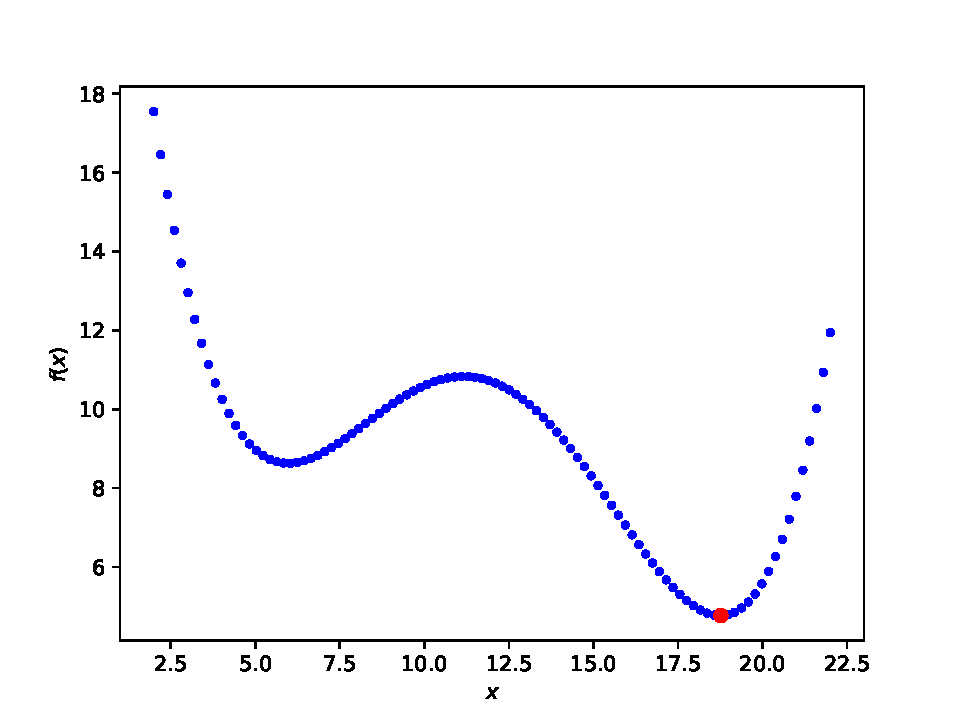
\includegraphics[width=0.8\textwidth]{./5_images/fig_grid_search_scalar.pdf} 
		\caption{Pesquisa em grade com número escalar}
		\label{fig:grid_search_scalar}
		\makebox[\width]{Fonte: Autor}
	\end{center}
\end{figure}

Ainda neste método, casos onde há uma maior quantidade de $x$ ($x_1$, $x_2$, \dots)
deve-se utilizar laços aninhados para que a varredura de todas as possibilidades
possa ser feita. 

Como exemplo, minimizemos a \cref{eq:grid_search_vect_no_bounds}, sendo
$0 \leq x_1 \leq 2$ e $1 \leq x_2 \leq 3$.

\begin{equation}
	\label{eq:grid_search_vect_no_bounds}
	f(x) = (x_1 - 1)^2 + (x_2 - 2)^2 + 0,5
\end{equation}

Neste caso, sem muito esforço notamos que
$f_{min} = 0,5$, $x_{1_{opt}} = 1$ e $x_{2_{opt}} = 2$.\footnote{
	O código-fonte em Python para este cálculo pode ser encontrado no
	\cref{ch:codigos_extras}, código \ref{lst:grid_search_vectorial}.}
Porém se a restrição da \cref{eq:grid_search_vect_bounds} for aplicada
encontramos os valores descritos nas equações descritas na \cref{eq:grid_search_vect_bounds_output}.

\begin{equation}
	\label{eq:grid_search_vect_bounds}
	f(x) = x_1 - x_2 + 1,5 \leq 0
\end{equation}

% \begin{subequations}
% 	\label{equ_grid_search_vect_bounds_output}
% 	\begin{align}
% 		f_{min} = 0,628 \\
% 		x_{1_{opt}} = 0,748 \\
% 		x_{2_{opt}} = 2,25
% 	\end{align}
% \end{subequations}

\begin{equation}
	\label{eq:grid_search_vect_bounds_output}
	\begin{aligned}
		f_{min} = 0,628 \\
		x_{1_{opt}} = 0,748 \\
		x_{2_{opt}} = 2,25
	\end{aligned}
\end{equation}

As figuras \ref{fig:grid_search_vectorial_nobounds} e \ref{fig:grid_search_vectorial_withbounds}
mostram a função custo (outra forma de chamarmos a função objetivo) sem restrição e com a
restrição descrita pela \cref{eq:min_restr_desigualdade}, respectivamente.

\begin{figure}[h]
    \centering
    \begin{minipage}{0.45\textwidth}
        \centering
        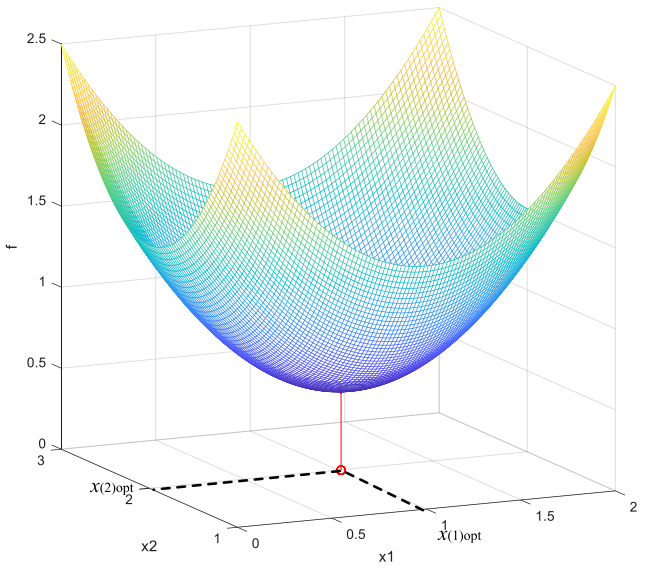
\includegraphics[width=0.9\textwidth]{./5_images/fig_grid_search_vectorial1.png} 
		\caption{Pesquisa em grade com duas variáveis e sem restrição}
		\label{fig:grid_search_vectorial_nobounds}
		Fonte: \citeonline{Haugen2018}
    \end{minipage}\hfill
    \begin{minipage}{0.45\textwidth}
        \centering
        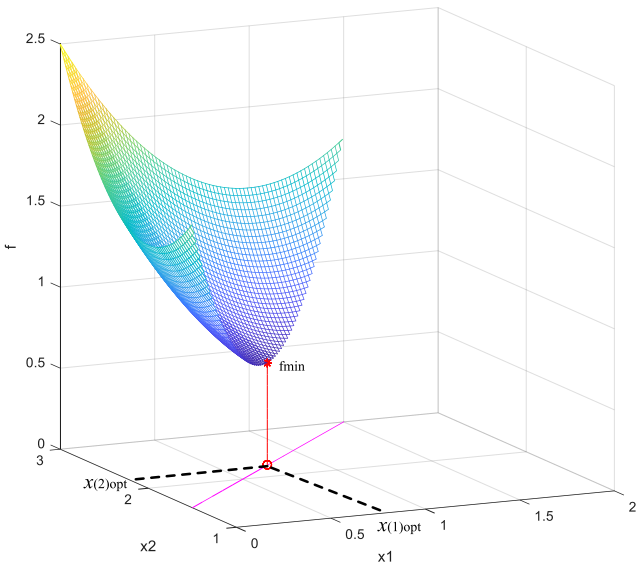
\includegraphics[width=0.9\textwidth]{./5_images/fig_grid_search_vectorial2.png} 
		\caption{Pesquisa em grade com duas variáveis e com restrição}  
		\label{fig:grid_search_vectorial_withbounds}		      
		Fonte: \citeonline{Haugen2018}
	\end{minipage}
\end{figure}

\subsection{Método de busca de descidas mais íngrimes}

Este método consiste em estimar o próximo valor de $x$ baseando-se na deriavada
da função custo calculada em $x$. Exemplificando para um caso escalar podemos dizer que
o próximo valor de $x$, isto é, $x_{k+1}$ será dado por:

\begin{align}
	\label{eq:steepest_decent_xk1}
	x_{k+1} &= x_k + \Delta x_k \\ 
	\Delta x_k &= -K f'(x_k)
\end{align}

\noindent
Onde: \\
$x_k$ = $x$ atual \\
$\Delta x_k$ = diferença entre $x_k$ e $x_{k+1}$ \\
$K$ = fator multiplicador do incremento \\
$f'(x_k)$ = derivada (ou gradiente) da função custo calculada em $x_k$ \newline

A derivada $f'(x_k)$ indica quão inclinada está a função custo no ponto $x_k$,
assim sendo o fator $K$ determina o peso que essa inclinação terá para o cálculo
do próximo valor de $x$.

A \cref{fig:steepest_decent_slope} mostra graficamente a influência da derivada
da função custo na amplitude de $\Delta x_k$ entre iterações.

\begin{figure}
	\begin{center}
		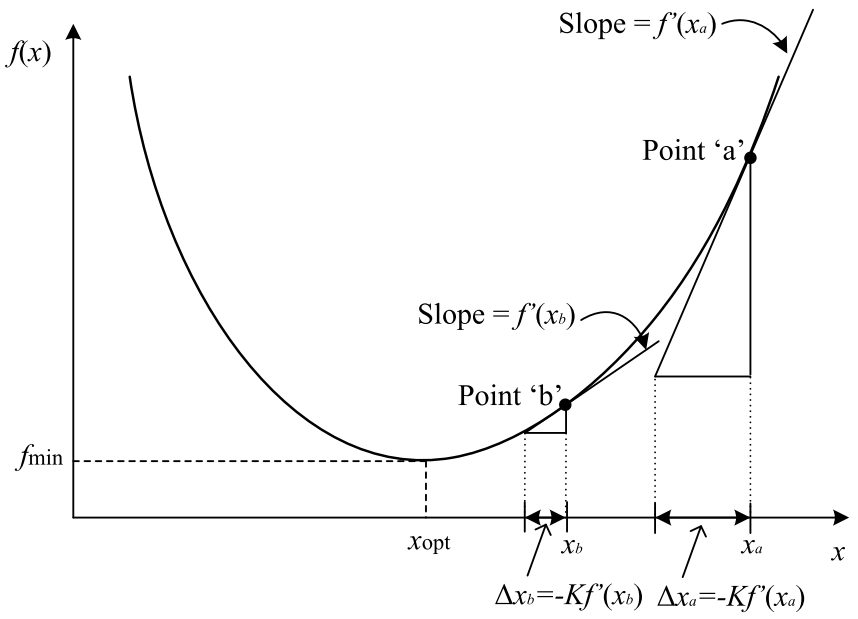
\includegraphics[width=0.75\textwidth]{./5_images/fig_steepest_decent_slope.png} 
		\caption{Influência de $f'(x_k)$ no cálculo de $x_{k+1}$ no método de descidas mais íngrimes}
		\label{fig:steepest_decent_slope}
		\makebox[\width]{Fonte: \citeonline{Haugen2018}}
	\end{center}
\end{figure}


\subsection{Método de Newton}

método de newton

\subsection{Otimizadores de programação não-linear (NLP)}

NLP

\section{Algumas aplicações de otimização}

\subsection{Estimação de parâmetros}

estimação de param

\subsection{Moving Horizon Estimation}

MHE

\subsection{Model Predictive Control}

MPC

% \chapter{Controle Preditivo}
\label{ch:controle_preditivo}

% =====================================================================================================
% ============================================= Section ===============================================
% =====================================================================================================
\section{Introdução}

% TODO: Alguma intro

% =====================================================================================================
% ============================================= Section ===============================================
% =====================================================================================================
\section{Cronologia}
\label{sec:cronologia}

% TODO: Cronologia

% =====================================================================================================
% ============================================= Section ===============================================
% =====================================================================================================
\section{Elementos do controle preditivo}
\label{sec:elementos_do_controle_preditivo}

% TODO: Apresentacão

% .....................................................................................................
% ............................................ Subsection .............................................
% .....................................................................................................
\subsection{Modelo do processo}
\label{subsec:modelo_do_processo}

% TODO: Modleo 

% .....................................................................................................
% ............................................ Subsection .............................................
% .....................................................................................................
\subsection{Função Objetivo}
\label{subsec:funcao_objetivo}

% TODO: fun obj

% .....................................................................................................
% ............................................ Subsection .............................................
% .....................................................................................................
\subsection{Lei de Controle}
\label{subsec:lei_de_controle}

% TODO: lei de controle

% =====================================================================================================
% ============================================= Section ===============================================
% =====================================================================================================
\section{As diferentes estratégias do controle preditivo}
\label{sec:diferentes_estrategias_controle_preditivo}

% TODO: estrategias

% =====================================================================================================
% ============================================= Section ===============================================
% =====================================================================================================
\section{Estabilidade}
\label{sec:estabilidade}

% TODO: estabilidade

% .....................................................................................................
% ............................................ Subsection .............................................
% .....................................................................................................
\subsection{Controle Preditivo com Horizonte de Predição Infinito}
\label{subsec:controle_preditivo_com_horizonte_preditivo_infinito}

% TODO: Controle de predicao infiinito

% .....................................................................................................
% ............................................ Subsection .............................................
% .....................................................................................................
\subsection{Controle Preditivo Não-Linear}
\label{subsec:controle_preditivo_nao_linear}

% TODO: Não-linear

% =====================================================================================================
% ============================================= Section ===============================================
% =====================================================================================================
\section{Análise Complementar dos Sistemas de Controle}
\label{sec:analise_complementar_dos_sistemas_de_controle}

% TODO: analise complementar

% .....................................................................................................
% ............................................ Subsection .............................................
% .....................................................................................................
\subsection{Representação no Espaço de Estados}
\label{subsec:representacao_no_espaco_de_estados}

% TODO: Espaço de Estados	% Reinserir quando capitulo estiver pronto (capítulo abandonado)

\chapter{Modelo Preditivo de Controle}
\label{cap_mpc}

\section{Introdução}

intro

\section{Algoritmos}

algo

\subsection{LQG}

LQG

\subsection{IDCOM}

IDCOM

\subsection{DMC}

DMC

\subsection{QDMC}

QDMC

\subsection{IDCOM-M, HIECON, SMCA e SMOC}

IDCOM-M

\subsection{DMC-plus e RMPCT In}

DMC-plus

% PARTE MATERIAIS E MÉTODOS
\part{Materiais e métodos}

\newacronym{tclab}{TCLab}{\textit{Temperature Control Lab}}

\chapter{Planta piloto}
\label{ch:planta_piloto}

O sistema experimental usado para o projeto de ações de controle é uma mini planta piloto chamada \acrlong{tclab}
(do inglês, Laboratório de Controle de Temperatura), ou apenas \acrshort{tclab}\footnote{                       % footnote
    Maiores informações sobre o \acrshort{tclab} podem ser encontrados em \href{http://apmonitor.com/heat.htm}{http://apmonitor.com/heat.htm}.
}. Esta planta foi desenvolvida na \textit{Brigham Young University} (BYU) e apresentada pela primeira vez no
\textit{2017 ASEE Summer School}, na \textit{North Carolina State University} (NCSU). Foi desenvolvida com o
propósito de facilitar o acesso de estudantes a um laboratório de testes de controle.

Esta mini planta é essencialmente um \textit{shield} para Arduino\footnote{
    Arduino é uma plataforma de prototipagem eletrônica de hardware livre e de placa única, projetada com um    % footnote
    microcontrolador Atmel AVR com suporte de entrada/saída embutido.                                           % footnote
} contendo 2 aquecedores e 2 sensores de temperatura, mostrado na \cref{fig:tclab}. A energia dos aquecedores é
transferida através de condução, convecção e radiação até os sensores de temperatura. Tanto o controle da
potência dos aquecedores quanto as medições realizadas pelos sensores são efetuados através do Arduino.

O \acrshort{tclab} possibilita fazer a programação do controle da mini planta utilizando linguagem Python,
\acrshort{matlab} ou Simulink.

\begin{figure}[h]
	\caption{Laboratório de Controle de Temperatura}
	\begin{center}
		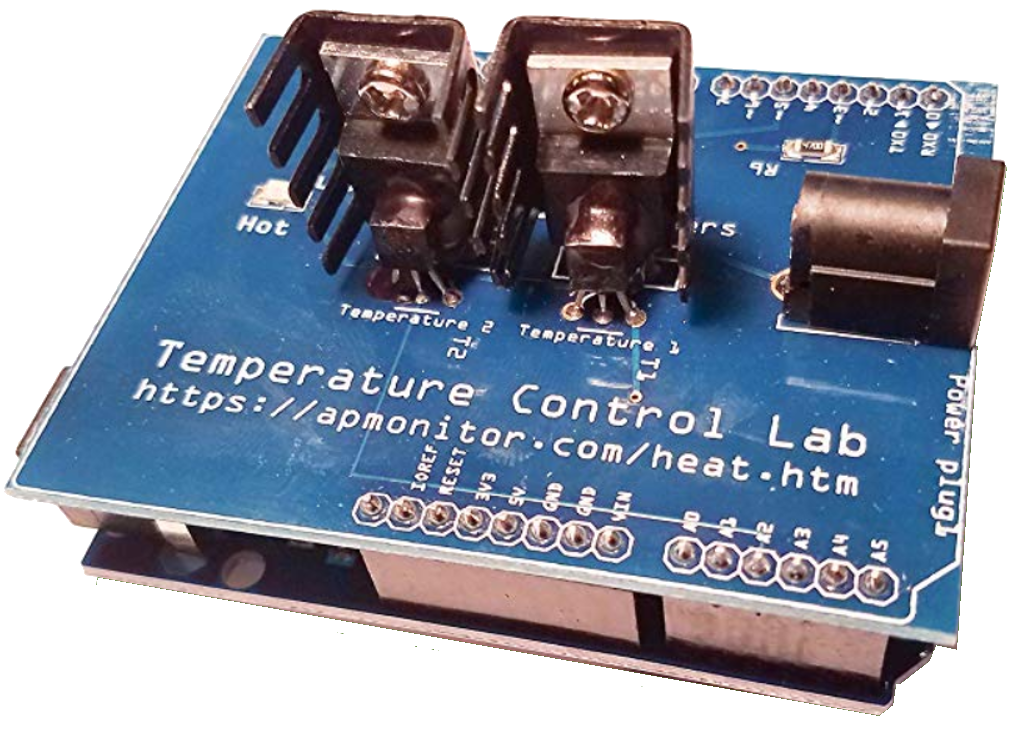
\includegraphics[width=0.55\textwidth]{./5_images/tclab.png} 
		\label{fig:tclab}
	\end{center}
	\centering
	\makebox[\width]{Fonte: ?????}  % TODO Corrigir autor
\end{figure}

% =====================================================================================================
% ============================================= Section ===============================================
% =====================================================================================================
\section{Modelagem da planta piloto}
\label{sec:modelagem_da_planta_piloto}

% TODO Adicionar modelagem descrita no http://apmonitor.com/pdc/index.php/Main/ArduinoModeling e nos Labs A e B

\newacronym{prbs}{PRBS}{\textit{Pseudo-Random Binary Signal}}
\newacronym{arma}{ARMA}{\textit{Auto-Regressive Moving Average}}
\newacronym{gbn}{GBN}{\textit{Generalized Binary Noise}}
\newacronym{ar}{AR}{Modelo autorregressivo}
\newacronym{arx}{ARX}{Modelo autorregressivo com entrada exógena}
\newacronym{armax}{ARMAX}{Modelo autorregressivo com média móvel e entrada exógena}
\newacronym{aic}{AIC}{Critério de informação de Akaike}
\newacronym{oe}{OE}{\textit{Output-Error}}
\newacronym{bj}{BJ}{Box-Jenkins}
\newacronym{nlarx}{NLARX}{ARX não-linear}
\newacronym{tf}{TF}{Função de transferência}
\newacronym{ss}{SS}{Espaço de estados}

\chapter{Modelagem experimental}
\label{ch:modelagem_experimental}

Segundo \citeonline{Gevers2006} a teoria de identificação de sistemas data da década de 60 e as duas
principais técnicas utilizadas na identificação de sistemas atualmente (método de identificação por
subespaço de estados e método do erro de predição) tiveram suas bases estruturadas com os trabalhos
de \apudonline{Ho1966}{Gevers2006} e de \apudonline{Astrom1965}{Gevers2006}.

De acordo com \apudonline{Dunia2008}{Pracek2012} a identificação do sistema permite que simulações
sejam desenvolvidas de modo a garantir um melhor desempenho dos sistemas de controle projetados.

As etapas para a identificação de um sistema, segundo \citeonline{Aguirre2015} são:
\begin{itemize}
    \item Testes dinâmicos e coleta de dados
    \item Escolha da representação matemática a ser utilizada
    \item Determinação da estrutura do modelos
    \item Estimação de parâmetros
    \item Validação do modelo
\end{itemize}

As seções a seguir detalham cada uma dessas etapas.

% =====================================================================================================
% ============================================= Section ===============================================
% =====================================================================================================
\section{Testes dinâmicos e coleta de dados}
\label{sec:testes_dinamicos_e_coleta_de_dados}

Esta etapa abrange os procedimentos necessários para geração do conjunto de dados que serão utilizados
para a identificação do sistema. Algumas das atividades realizadas nessa etapa são: escolha das variáveis,
definição dos sinais de excitação, definição do período de amostragem e execução de testes.
\cite{Aguirre2015}

% -----------------------------------------------------------------------------------------------------
% ------------------------------------------- subsection -------------------------------------------
% -----------------------------------------------------------------------------------------------------
\subsection{Período de amostragem}
\label{subsec:periodo_de_amostragem}

Segundo o teorema de Shannon, descrito por \citeonline{Aguirre2015}, "um sinal que não contenha componentes
de frequência acima de $1/2T_s$ pode ser determinado unicamente a partir de amostras de tal sinal separadas
por $T_s$", sendo $T_s$ o período de amostragem ou, como também é chamado, tempo de amostragem.

Na prática, contudo, um período de amostragem apenas 2 vezes maior que a frequência de interesse, como exigido
pelo teorema de Shannon, nem sempre é suficiente. Normalmente então escolhe-se uma frequência de amostragem
entre 5 e 10 vezes maior do que a maior do que tal frequência desejada \cite{Aguirre2015}. Por outro lado, do
ponto de vista numérico, se o intervalo de amostragem for muito curto, a estimação de parâmetros também
poderá se tornar malcondicionada \cite{Aguirre2015}.

Para a identificação da maior frequência de interesse do sistema analisado, alguns ensaios foram realizados\footnote{
    \textit{Scripts} utilizados no \cref{sec:tclabsp_tempo_de_subida}
}
excitando o Aquecedor 1 do \acrshort{tclabsp} em $50\%$ e aproximando a resposta em malha aberta dos
Sensores de Temperatura 1 e 2 para um sistema de primeira ordem, a fim de obter o valor do tempo de subida
($\tau$). Esse tempo de subida servirá de referência para o cálculo do período de amostragem.

\begin{figure}[h]
	\caption{Tempo de subida - Sensor de Temperatura 1}
	\begin{center}
		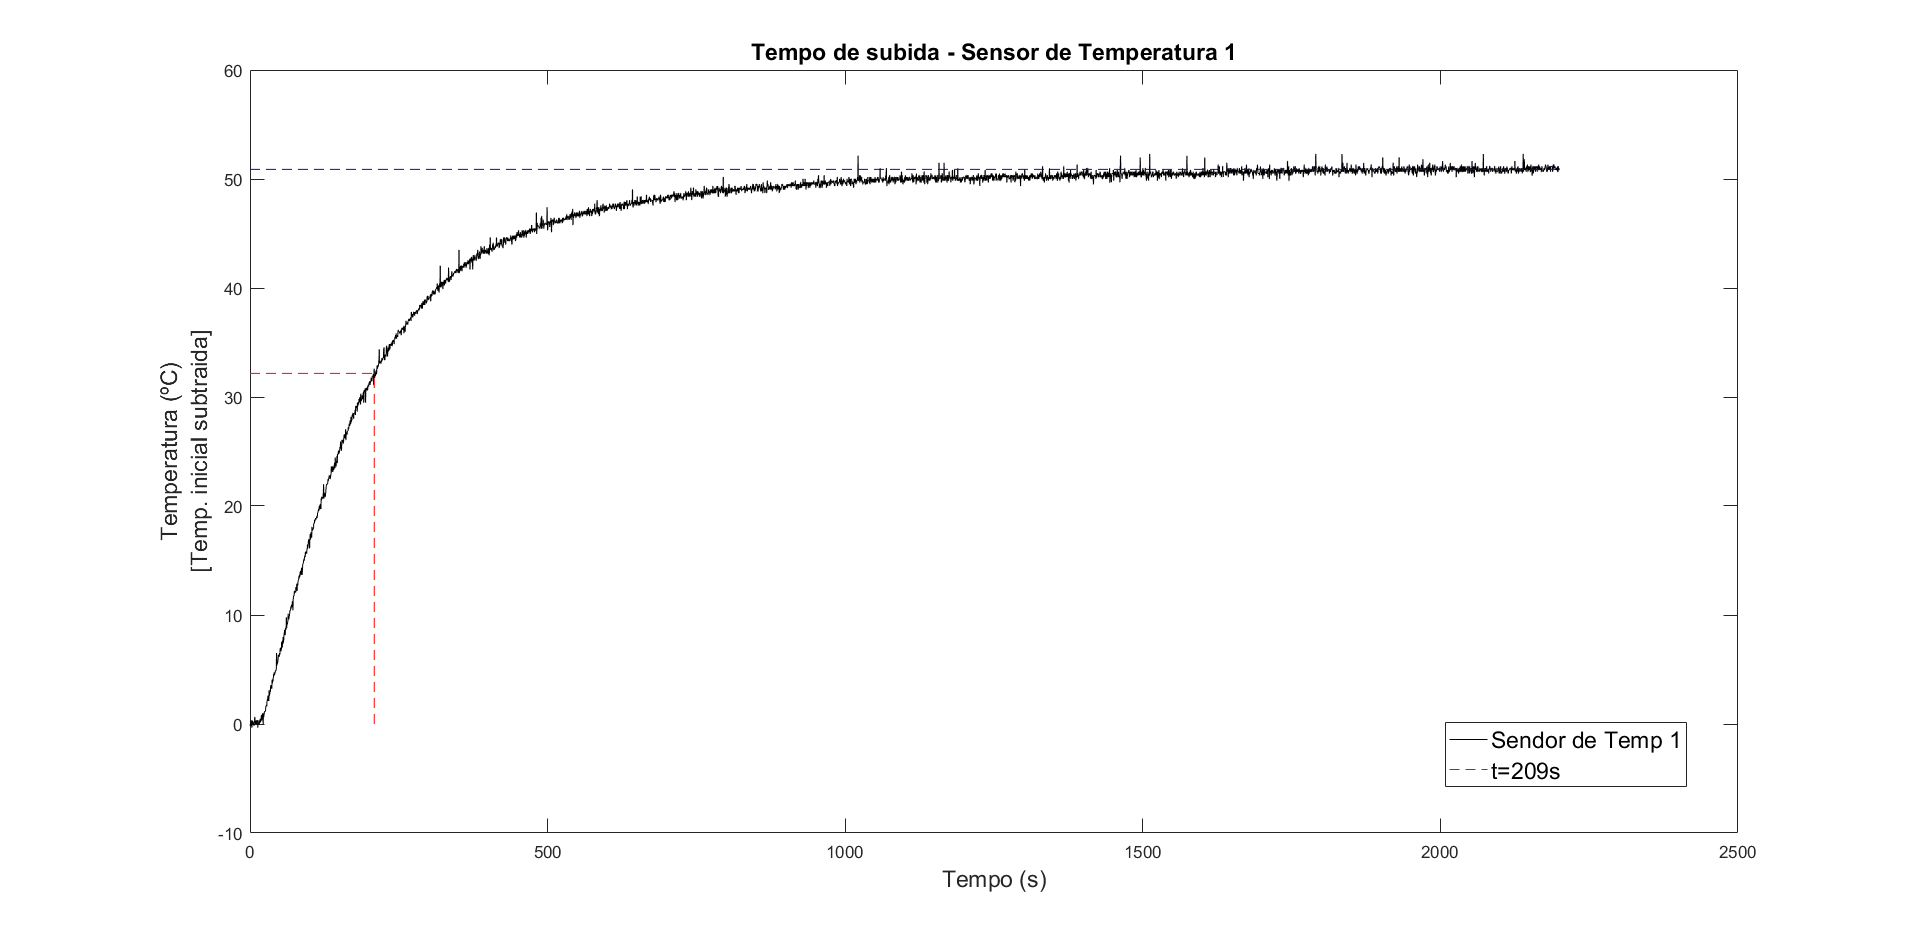
\includegraphics[width=0.95\textwidth]{./5_images/RiseTime-TempSensor1.png} 
		\label{fig:rise_time_sensor1}
	\end{center}
	\centering
	\makebox[\width]{Fonte: \citeonline{Prata2019}} 
\end{figure}

\begin{figure}[h]
	\caption{Tempo de subida - Sensor de Temperatura 2}
	\begin{center}
		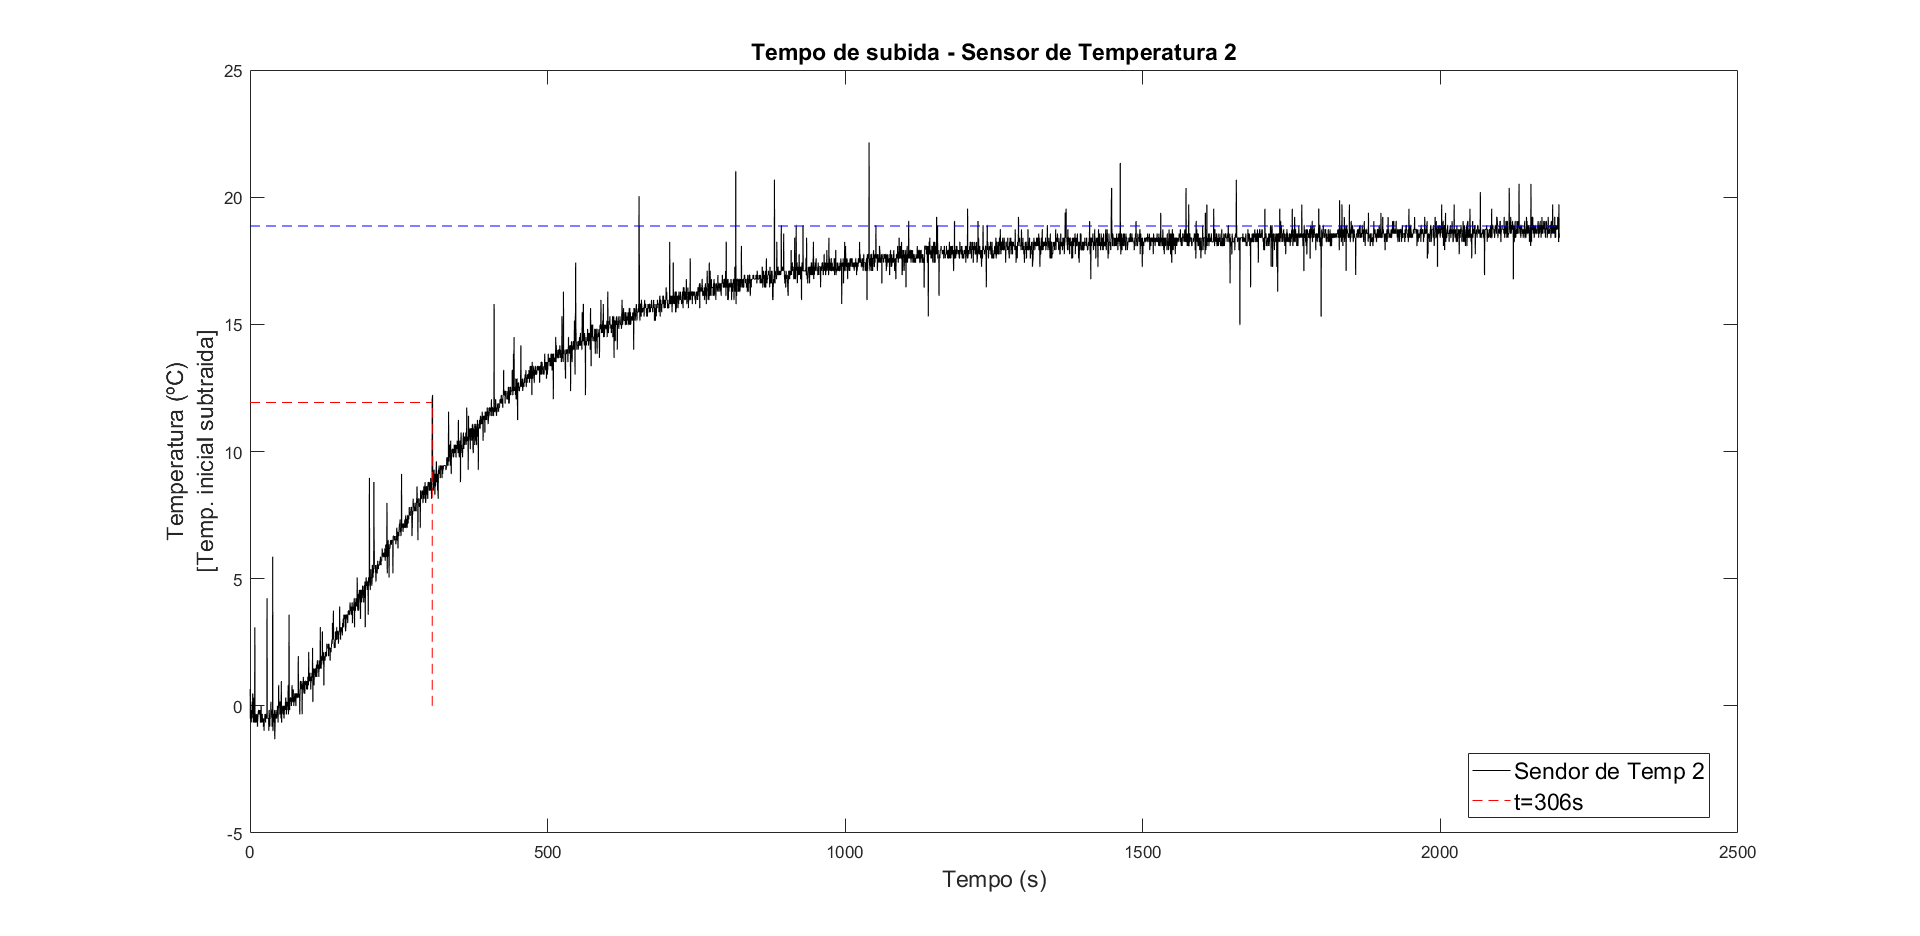
\includegraphics[width=0.95\textwidth]{./5_images/RiseTime-TempSensor2.png} 
		\label{fig:rise_time_sensor2}
	\end{center}
	\centering
	\makebox[\width]{Fonte: \citeonline{Prata2019}} 
\end{figure}

As \cref{fig:rise_time_sensor1,fig:rise_time_sensor2} mostram a resposta em malha aberta dos Sensores de
Temperatura 1 e 2, respectivamente, a uma entrada degrau no Aquecedor 1. Este ensaio foi realizado com
um período de amostragem de 0,5s, e com ele foi possível observar um tempo de subida $\tau_1 = 209s$ para
o Sensor 1 e $\tau_2 = 383s$ para o Sensor 2.
% TODO: Fazer mais ensaios com step 0 -> 50
% TODO: Recortar as imagens para remover bordas brancas

Seguindo a regra prática de \citeonline{Aguirre2015} onde $T_s$ deve ser entre 5 e 10 vezes maior que a
maior frequência desejada, então temos que $20.9s > T_s > 41.8s$.

Para os ensaios realizados neste trabalho, optou-se pela maior frequência de amostragem possível, como
mostrado na \cref{eq:sampling_time}.

\begin{equation}
	\label{eq:sampling_time}
	T_s = 20.9s
\end{equation}

Outra técnica também descrita por \citeonline{Aguirre2015} para a escolha da frequência de amostragem,
apesar de não ter sido escolhida, também foi testada e é descrita em maiores detalhes no
\cref{ch:sampling_time_using_autocorrelation}.

% -----------------------------------------------------------------------------------------------------
% ------------------------------------------- Subsection -------------------------------------------
% -----------------------------------------------------------------------------------------------------
\subsection{Sinais de excitação}
\label{subsec:sinais_de_excitacao}

% \acrshort{arma} - Média Móvel Auto-Regressiva (do inglês, \acrlong{arma})
A escolha dos sinais de entrada pode ter grande impacto nos dados coletados,
pois determinarão o ponto de operação do sistema e quais das suas características serão excitadas
durante o experimento \cite{Aguirre2015}.
Diversos tipos distintos de sinais podem ser utilizados. Entre os mais comuns destacam-se:
impulsivo; degrau; \acrshort{prbs} - Sinal Binário Pseudo-Aleatório (do inglês, \acrlong{prbs});
\acrshort{gbn} - Ruido Binário Generalizado (do inglês, \acrlong{gbn}); soma de senóides e etc \cite{Aguirre2015}.
Porém quando objetiva-se a identificação do sistema de onde os dados foram coletados, no geral
os métodos de identificação exigem que os sinais de entrada tenham um espectro de frequência
branco ou quase branco. Sinais aleatórios e pseudoaleatórios satisfazem essa condição \cite{Aguirre2015}.

Sinais \acrshort{prbs} são comumente usados na identificação de sistemas lineares, porém para sistemas
não-lineares tais sinais não são adequados, neste caso muitas vezes será desejável excitar o
sistema numa larga faixa de amplitudes a fim de poder observar suas características estáticas e dinâmicas
\cite{Aguirre2015}.

\begin{citacao}
    Características dinâmicas e estáticas que não forem excitadas não aparecerão nos dados. O que
    não estiver nos dados não pode ser identificado. Tal princípio é utilizado, por exemplo,
    quando um sistema é excitado em torno de um ponto de operação. Neste caso, como as não-linearidades
    não foram excitadas no teste, é possível, pelo menos em princípio, ajustar um modelo linear
    aos dados assim obtidos. \cite{Aguirre2015}
\end{citacao}

Segundo \citeonline{Aguirre2015} uma regra prática para a aplicação do sinal de excitação é,
tendo-se definido o tempo de amostragem (já discutido na \cref{subsec:periodo_de_amostragem}),
manter constante o valor escolhido aleatóriamente por um tempo, em torno de 3 a 5 intervalos de
amostragem.

Para a coleta dos sinais do \acrshort{tclabsp} foram aplicados tanto no Aquecedor 1 quanto no
Aquecedor 2 sinais de entrada aleatórios, mantidos constantes por um período de $3T_s$ a $5T_s$
(vide \cref{eq:sampling_time}). Contudo, antes dos sinais aleatórios serem aplicados aos
aquecedores, um sinal constante de $50\%$ foi aplicado a cada um deles por $1500s$ com o intuito
de estabilizá-los em um patamar onde as amplitudes dos sinais aleatórios aplicados tivessem
maior liberdade. A \cref{fig:simulink_coleta} mostra o modelo \textit{Simulink} utilizado para
a coleta dos dados e a \cref{fig:experiment_inputs} mostra os sinais de entrada aplicados nos
Aquecedores 1 e 2.

\begin{figure}[h]
	\caption{Modelo \textit{Simulink} para coleta de dados}
	\begin{center}
		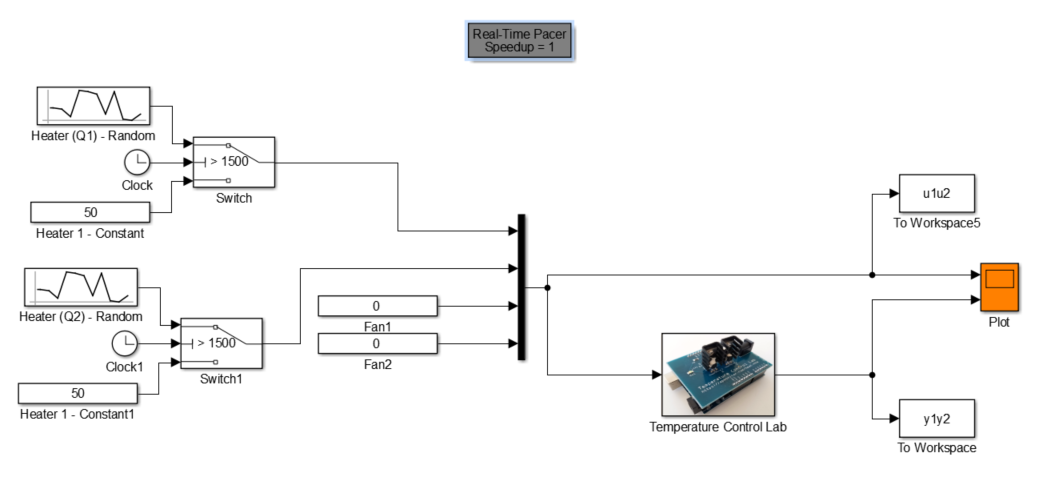
\includegraphics[width=0.85\textwidth]{./5_images/SimulinkColeta.png} 
		\label{fig:simulink_coleta}
	\end{center}
	\centering
	\makebox[\width]{Fonte: Autor} 
\end{figure}

\begin{figure}[h]
	\caption{Sinais de entrada nos Aquecedores 1 e 2}
	\begin{center}
		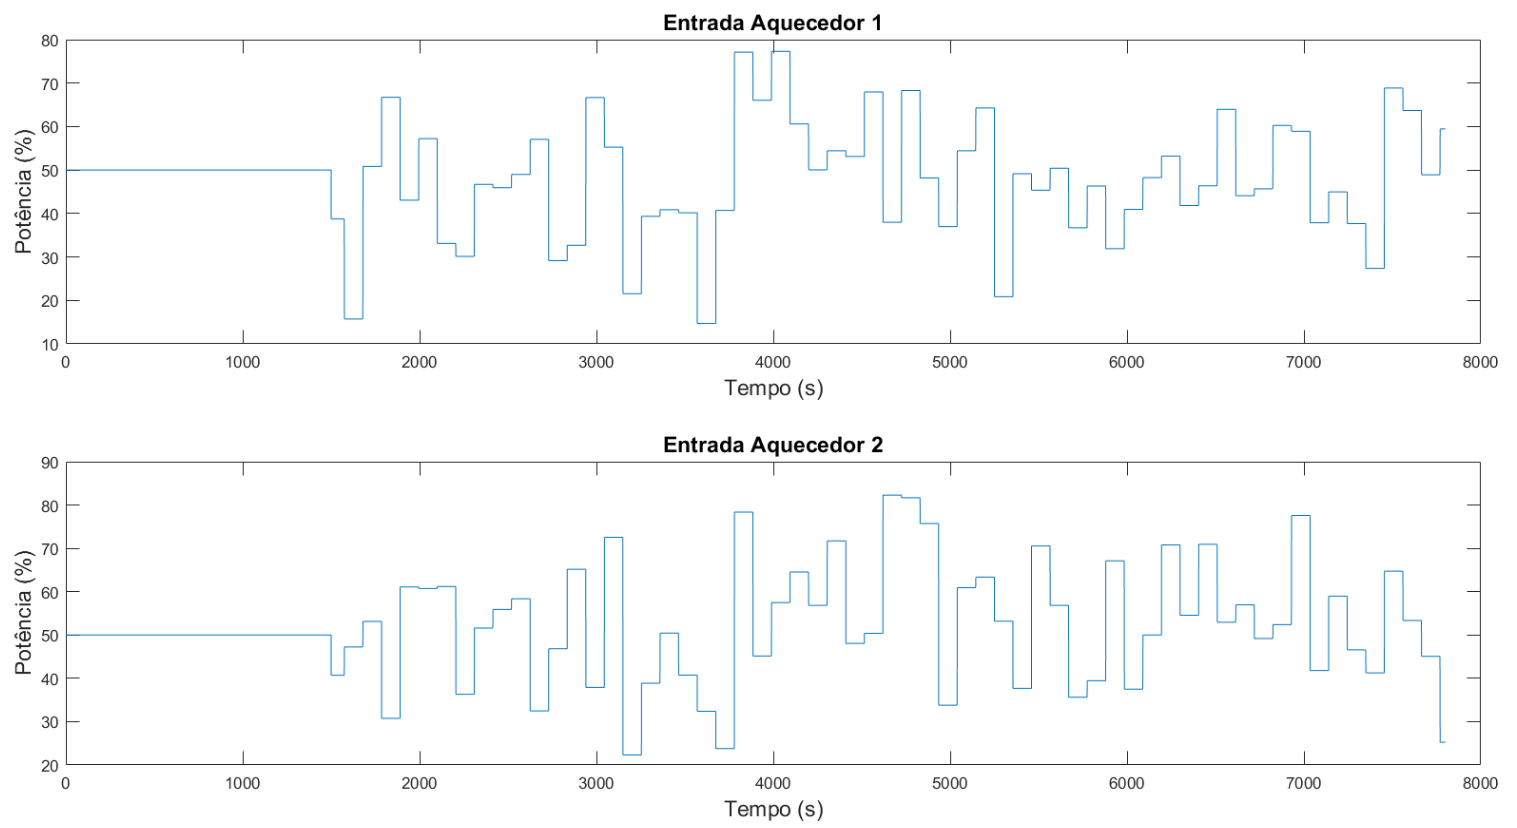
\includegraphics[width=0.95\textwidth]{./5_images/inputs_H1H2.png} 
		\label{fig:experiment_inputs}
	\end{center}
	\centering
	\makebox[\width]{Fonte: Autor} 
\end{figure}

% -----------------------------------------------------------------------------------------------------
% ------------------------------------------- Subsection -------------------------------------------
% -----------------------------------------------------------------------------------------------------
\subsection{Duração do experimento}
\label{subsec:duracao_do_experimento}

A duração do experimento, segundo \citeonline{Garcia2005}, deveria ser
a maior possível, uma vez que a variância das estimativas é proporcional ao inverso da duração do
experimento, porém sob o ponto de vista prático e experimental, a duração do experimento deveria ser
a menor possível para a obtenção de um modelo aceitável, pois ao longo do experimento o processo
estará sujeito a perturbações extras que podem impactar na operação da planta, na qualidade dos
produtos ou até na segurança do processo.

Cada um dos experimentos de coleta de dados do \acrshort{tclabsp} teve uma duração de $7800s$,
sendo que os $1500s$ iniciais foram utilizados para a estabilização do processo e os demais ($6300s$)
para as coletas. O critério utilizado para a determinação deste valor foi o de estimular a dinâmica
da planta aproximadamente $60x$ para cada um dos experimentos. Sabendo que os sinais de excitação
podem permanecer constantes por até $105s$ ($5T_s$), como mostrado na \cref{subsec:sinais_de_excitacao},
então temos a \cref{eq:experiment_duration}:

\begin{equation}
	\label{eq:experiment_duration}
	60 * 5T_s = \pmb{6}\pmb{3}\pmb{0}\pmb{0}\pmb{s}
\end{equation}

% .....................................................................................................
% ............................................ Section .............................................
% .....................................................................................................
\section{Definição do modelo experimental}
\label{sec:definicao_modelo_experimental}

Esta seção apresenta mais algumas características teóricas importantes na definição de um modelo
que represente o sistema simulado e ao final dela, a \cref{sec:modelo_experimental}
mostra a aplicação prática dessas características utilizando o conjunto de ferramentas do \acrshort{matlab}
para identificação de sistemas, o \textit{System Identification Toolbox\texttrademark}.

% -----------------------------------------------------------------------------------------------------
% ------------------------------------------- Subsection -------------------------------------------
% -----------------------------------------------------------------------------------------------------
\subsection{Escolha da representação matemática}
\label{subsec:escolha_da_representacao_matematica}

Existem diversas representações matemáticas distintas para modelos lineares, sendo que, segundo
\citeonline{Aguirre2015}, a mais utilizada é a função de transferência, porém \citeonline{Wang2009}
destaca que nos últimos anos tem se observado um aumento na popularidade dos modelos de espaço de
estados para desenvolvimento de controle preditivo. Para \citeonline{Aguirre2015} é importante ainda
salientar o modelo \acrshort{ar} (\acrlong{ar}), o modelo \acrshort{arx} (\acrlong{arx}) e
o modelo \acrshort{armax} (\acrlong{armax}).

\begin{citacao}
    \text{[...]} quando se trata da modelagem obtida por meios fenomenológicos é comum que se adote a base de
    tempo contínuo, em virtude de a maioria das leis da física serem expressas nesse tempo. Por sua vez,
    quando se trata de identificação de sistemas por processos experimentais, trabalha-se com amostras
    de dados coletados a cada intervalo de tempo, nesses casos usualmente adota-se o tempo discreto.
    \apud{Garcia2005}{Favaro2012}
\end{citacao}

% -----------------------------------------------------------------------------------------------------
% ------------------------------------------- Subsection -------------------------------------------
% -----------------------------------------------------------------------------------------------------
\subsection{Determinação da estrutura do modelos}
\label{subsec:determinacao_da_estrutura_do_modelo}

Determinar a ordem de um modelo é um dos aspectos mais importantes na determinação de sua estrutura,
uma vez que, caso sua ordem seja muito menor do que a ordem efetiva do sistema real, o modelo não
refletirá a completamente sua complexidade estrutural. Analogamente, escolher um modelo que a ordem
seja muito maior do que a necessária, provavelmente causará uma estimação de parâmetros mal condicionada.
\cite{Aguirre2015}

Neste trabalho será utilizado o \textit{critério de informação de Akaike} \apud{Akaike1974}{Aguirre2015}
(\acrshort{aic}), definido por:

\begin{equation}
	\label{eq:aic}
	AIC(n_\theta) = N \ln \left[ \sigma_{erro}^2 (n_\theta) \right] + 2n_\theta
\end{equation}

\noindent
Onde: 
\begin{itemize}
	\item $N$: é o número de dados
	\item $\sigma_{erro}^2 (n_\theta)$: é a variância dos resíduos
	\item $n_\theta = \mathrm{dim}[\hat{\theta}]$: é o número de parâmetros do modelo
\end{itemize}

Segundo \citeonline{Aguirre2015} a utilização deste critério na escolha da estrutura do modelo se justifica
pois à medida que termos são incluídos no modelo, o número de graus de liberdade aumenta, permitindo
um ajuste de dados mais exato. Resumidamente, a primeira parcela da equação quantifica a diminuição
da variância dos resíduos resultante da inclusão de um termo, ao passo que a segunda parcela penaliza
a inclusão de cada termo.

O índice \acrshort{aic}($n_\theta$) normalmente atinge um mínimo para um determinado número de parâmetros
no modelo $n_{\theta}^*$, e, ainda segundo \citeonline{Aguirre2015}, do ponto de vista do critério utilizado,
esse número de parâmetros é ótimo.

% -----------------------------------------------------------------------------------------------------
% ------------------------------------------- Subsection -------------------------------------------
% -----------------------------------------------------------------------------------------------------
\subsection{Estimação de parâmetros}
\label{subsec:estimacao_de_parametros}

A estimação de parâmetros, segundo \apudonline{Eykhoff1974}{Favaro2012} é a determinação experimental
de valores de parâmetros que governam a dinâmica e/ou o comportamento não-linear, assumindo que a
estrutura do modelo seja conhecida.

Essa etapa começa com a escolha do algoritmo a ser utilizado \cite{Aguirre2015}. Dentre eles, os
mais amplamente empregados na literatura são: método da análise de frequência; método da resposta
transitória e método dos mínimos quadrados \cite{Favaro2012}.

Como será visto na \cref{sec:modelo_experimental}, neste trabalho diversas representações matemáticas
distintas foram testadas, e para cada uma delas foi utilizada uma função do \acrshort{matlab} para 
a estimação automática de parâmetros. A \cref{tab:param_est_functions} identifica as funções
utilizadas em cada uma das representações distintas\footnote{
    Documentações das funções disponíveis em:

    $\mathtt{tfest}$ - \url{https://www.mathworks.com/help/ident/ref/tfest.html}

    $\mathtt{ssest}$ - \url{https://www.mathworks.com/help/ident/ref/ssest.html}

    $\mathtt{arx}$ - \url{https://www.mathworks.com/help/ident/ref/arx.html}

    $\mathtt{armax}$ - \url{https://www.mathworks.com/help/ident/ref/armax.html}

    $\mathtt{oe}$ - \url{https://www.mathworks.com/help/ident/ref/oe.html}

    $\mathtt{bj}$ - \url{https://www.mathworks.com/help/ident/ref/bj.html}
}.

\begin{table}[h]
	\centering
	\caption{Funções para a estimação de parâmetros}
	\label{tab:param_est_functions}
	\begin{tabular}{ll} \toprule
		{Representação matemática}		                                & {Função}				                    \\ \midrule
		Função de transferência		                                    & $\mathtt{tfest}$                          \\
		Espaço de estados   		                                    & $\mathtt{ssest}$                          \\
		\acrshort{arx}		                                            & $\mathtt{arx}$                            \\
		\acrshort{armax}		                                        & $\mathtt{armax}$                          \\
		Erro de saída (\acrshort{oe}, do inglês \acrlong{oe})		    & $\mathtt{oe}$                             \\
		\acrlong{bj} (\acrshort{bj})             	                    & $\mathtt{bj}$                             \\ \bottomrule
	\end{tabular}
	\caption*{Fonte: Autor}
\end{table}

% -----------------------------------------------------------------------------------------------------
% ------------------------------------------- Subsection -------------------------------------------
% -----------------------------------------------------------------------------------------------------
\subsection{Validação do modelo}
\label{subsec:validacao_do_modelo}

Em problemas de validação, a questão é tentar determinar se um dado modelo é válido ou não e para isso,
deve-se simulá-lo sem qualquer ajuste adicional e compará-lo a dados medidos em testes diferentes daquele
usado no desenvolvimento da sintonia do mesmo. A motivação para tal cuidado deve-se ao fato de desejar-se
saber o quão geral é o modelo. Portanto, esta divisão entre os dados de treinamento e de validação refere-se
à \textit{capacidade de generalização do modelo} \cite{Aguirre2015}.

A proporção entre dados de treinamento e validação utilizada neste trabalho é de 60\% para dados de treinamento
e 40\% para validação. Para realizar a comparação entre o modelo obtido e os dados de validação, utilizou-se
a função \texttt{compare} no \acrshort{matlab}.

Esta função \texttt{compare} avalia o quanto o modelo obtido se encaixa aos dados de validação calculando
o erro do quadrado médio da raiz normalizada, assim como descrito na \cref{eq:nrmse} a seguir:

\begin{equation}
	\label{eq:nrmse}
	\mathrm{fit} = 100 \left( 1 - \frac{ \| y - \hat{y} \| }{ \| y - \mathrm{média}(y) \| } \right)
\end{equation}

\noindent
Onde: 
\begin{itemize}
	\item $y$: são os dados de validação
	\item $\hat{y}$: são os dados do modelo
\end{itemize}

Também neste trabalho aplica-se o teste de \textit{análise de resíduos} dos modelos estudados e a motivação
para tal pode ser melhor compreendida nas palavras de \citeonline{Aguirre2015} a seguir:

\begin{citacao}
    \text{[...]} Do ponto de vista da validação de modelos, a motivação de se verificar quão são aleatórios
    os resíduos pode ser entendida lembrando que os resíduos são a parte dos dados que o modelo não
    consegue explicar. Exigir que o modelo explique os dados em todos os seus detalhes é, no mínimo,
    ingênuo. Mas quanto dos dados precisa ser explicado? O modelo deve explicar \textit{tudo que for
    explicável nos dados}. Se isso ocorrer, então os resíduos conterão apenas aquilo que não é explicável e,
    portanto, serão brancos. Assim, se os resíduos forem brancos, não há informação útil neles, ou seja,
    o modelo explicou tudo que era possível explicar. \text{[...]} 
\end{citacao}

Para tal teste utiliza-se a função \texttt{resid} no \acrshort{matlab}.

% -----------------------------------------------------------------------------------------------------
% ------------------------------------------- Section -------------------------------------------
% -----------------------------------------------------------------------------------------------------
\section{Modelos experimentais}
\label{sec:modelo_experimental}

Esta seção apresenta maiores detalhes práticos dos procedimentos descritos nas 
\crefrange{subsec:escolha_da_representacao_matematica}{subsec:validacao_do_modelo} e os
\textit{scripts} de \acrshort{matlab} utilizados para a obtenção dos resultados também serão
apresentados e discutidos ao longo do texto.

Após as coletas de dados descritas das
\crefrange{sec:testes_dinamicos_e_coleta_de_dados}{subsec:duracao_do_experimento}
preparou-se então no \acrshort{matlab} um objeto do tipo \texttt{iddata} contendo os dados dos aquecedores
e dos sensores de temperatura do \acrshort{tclabsp}.
Esses dados foram divididos em 2 grupos: identificação e validação, como já visto na \cref{subsec:validacao_do_modelo}.
As entradas e saídas do sistema, subdivididas nesses 2 grupos, foram criadas a partir do código-fonte
\ref{lst:tclabsp-model-iddata} e podem ser observadas na \cref{fig:tclabsp-model-IOs}.

\begin{figure}[h]
	\caption{Entradas e saídas coletadas em ensaios no \acrshort{tclabsp}}
	\begin{center}
		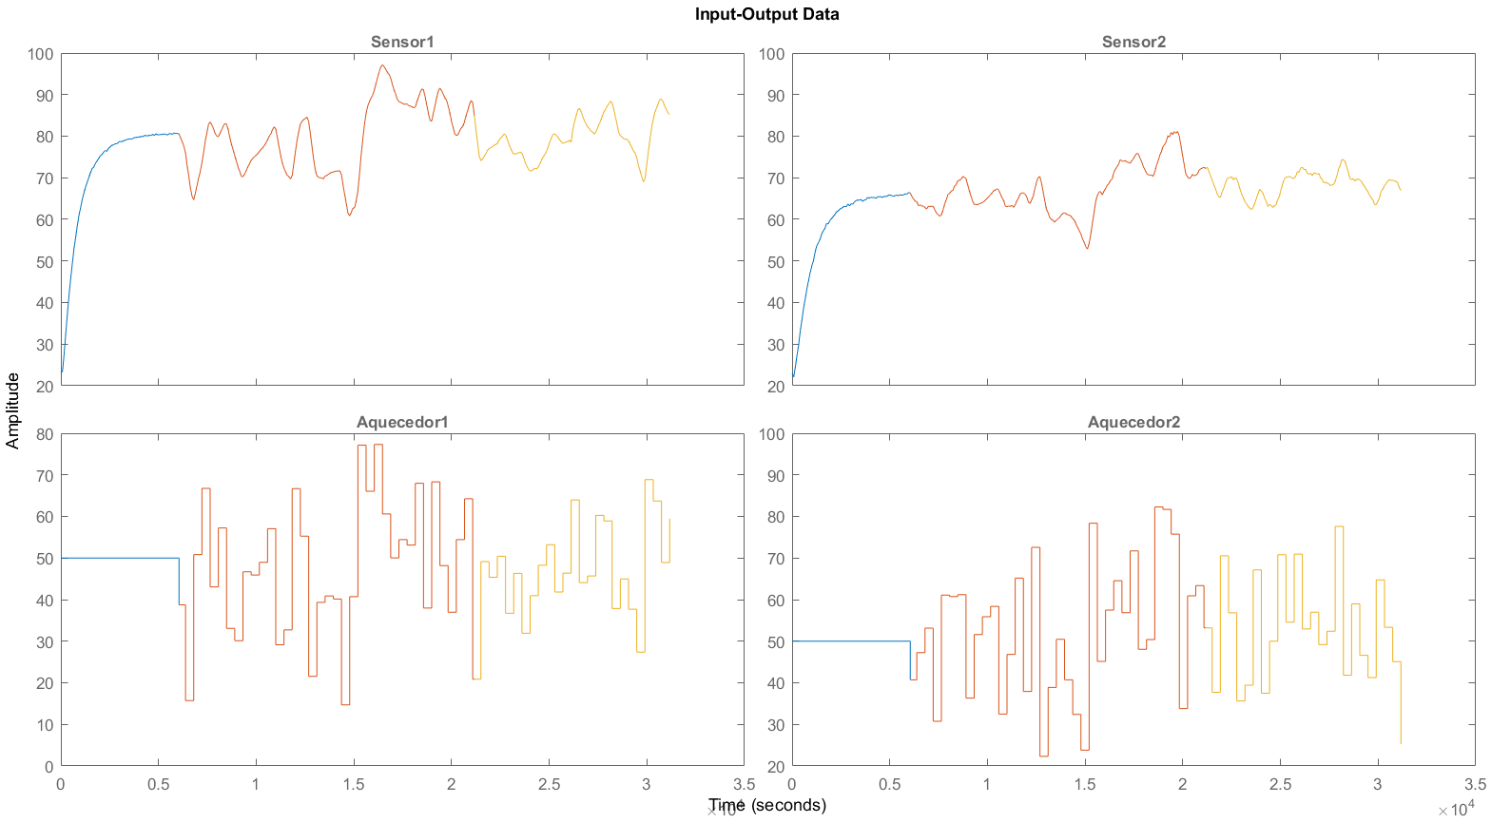
\includegraphics[width=1.00\textwidth]{./5_images/tclabsp-model-IOs.png} 
		\label{fig:tclabsp-model-IOs}
	\end{center}
	\centering
	\makebox[\width]{Fonte: Autor} 
\end{figure}

Na \cref{fig:tclabsp-model-IOs} é possível observar 3 conjuntos de dados distintos, indicados pelas cores 
azul, vermelho e laranja. Os dados em \textbf{azul} foram descartados, pois representam o período de 
estabilização do sistema em 50\% dos aquecedores. Os dados em \textbf{vermelho} e \textbf{laranja} representam
os dados de identificação e validação, respectivamente.

\lstinputlisting[	
	caption={Criação dos conjuntos de identificação e validação para o sistema \acrshort{tclabsp}},
	captionpos=t,
    label={lst:tclabsp-model-iddata},
    firstline=1,
    lastline=55,
    language=Matlab,
	style=Matlab_lang]
	{D:/Repos/TCLabSP/Simulink (MATLAB R2016a)/02-ModeloExperimental/RunMe.m}
	\begin{center}
		\makebox[\width]{Fonte: Autor}
    \end{center}
% TODO: Substituir endereço do arquivo

Com o intuito fazer diversos testes e de avaliar muitos modelos diferentes, utilizou-se um
\textit{script} para a criação automática de modelos experimentais baseados nos dados mostrados
na \cref{fig:tclabsp-model-IOs}. Este \textit{script} utiliza as funções descritas na \cref{tab:param_est_functions}
e seu código-fonte pode ser visto no \cref{sec:tclabsp-models-creation}. 
A \cref{tab:tclabsp-models-description} apresenta a quantidade de modelos que foram gerados a partir dele.

\begin{table}[h]
	\centering
	\caption{Modelos experimentais do \acrshort{tclabsp}}
	\label{tab:tclabsp-models-description}
	\begin{tabular}{ll} \toprule
		{Representação matemática}		                                & {Quantidade}          \\ \midrule
		Função de transferência		                                    & $10.000$              \\
		Espaço de estados   		                                    & $10$                  \\
		\acrshort{arx}		                                            & $9$                   \\
		\acrshort{armax}		                                        & $36$                  \\
		\acrshort{oe}													& $10$                  \\
		\acrshort{bj}                                   				& $160$                 \\ \bottomrule
	\end{tabular}
	\caption*{Fonte: Autor}
\end{table}

% _____________________________________________________________________________________________________
% ___________________________________________ Paragraph _______________________________________________
% _____________________________________________________________________________________________________
\paragraph*{\textbf{Modelos experimentais de função de transferência}}
\label{par:modelos_experimentais_tf}

Os modelos experimentais criados na forma de função de transferência foram obtidos a partir de diversas combinações
entre a quantidade de pólos e zeros nos subsistemas existentes entre os Sensores 1 e 2, e entre os Aquecedores 1 e 2.
Essas combinações são descridas na \cref{tab:tclabsp-models-tf}.

\begin{table}[h]
	\centering
	\caption{Modelos experimentais - Função de transferência}
	\label{tab:tclabsp-models-tf}
	\begin{tabular}{l|l|l|}
        \cline{2-3}
                                                & \textbf{Aquecedor 1}                                                      & \textbf{Aquecedor 2}                                                      \\ \hline
        \multicolumn{1}{|l|}{\textbf{Sensor 1}} & \begin{tabular}[c]{@{}l@{}}pólos: de 2 a 5\\ zeros: de 1 a 4\end{tabular} & \begin{tabular}[c]{@{}l@{}}pólos: de 2 a 5\\ zeros: de 1 a 4\end{tabular} \\ \hline
        \multicolumn{1}{|l|}{\textbf{Sensor 2}} & \begin{tabular}[c]{@{}l@{}}pólos: de 2 a 5\\ zeros: de 1 a 4\end{tabular} & \begin{tabular}[c]{@{}l@{}}pólos: de 2 a 5\\ zeros: de 1 a 4\end{tabular} \\ \hline
    \end{tabular}
	\caption*{Fonte: Autor}
\end{table}

Para cada uma das combinações possíveis descritas na \cref{tab:tclabsp-models-tf} foi criado um modelo utilizando o
conjunto de dados de identificação. Esses modelos foram testados com o conjunto de dados de validação através da \cref{eq:nrmse}
e o resultado destes testes, juntamente com o critério de \acrshort{aic}, podem ser observados na \cref{fig:tclabsp-models-tf}.

\begin{figure}[h]
	\caption{Modelos experimentais de função de transferência}
	\begin{center}
		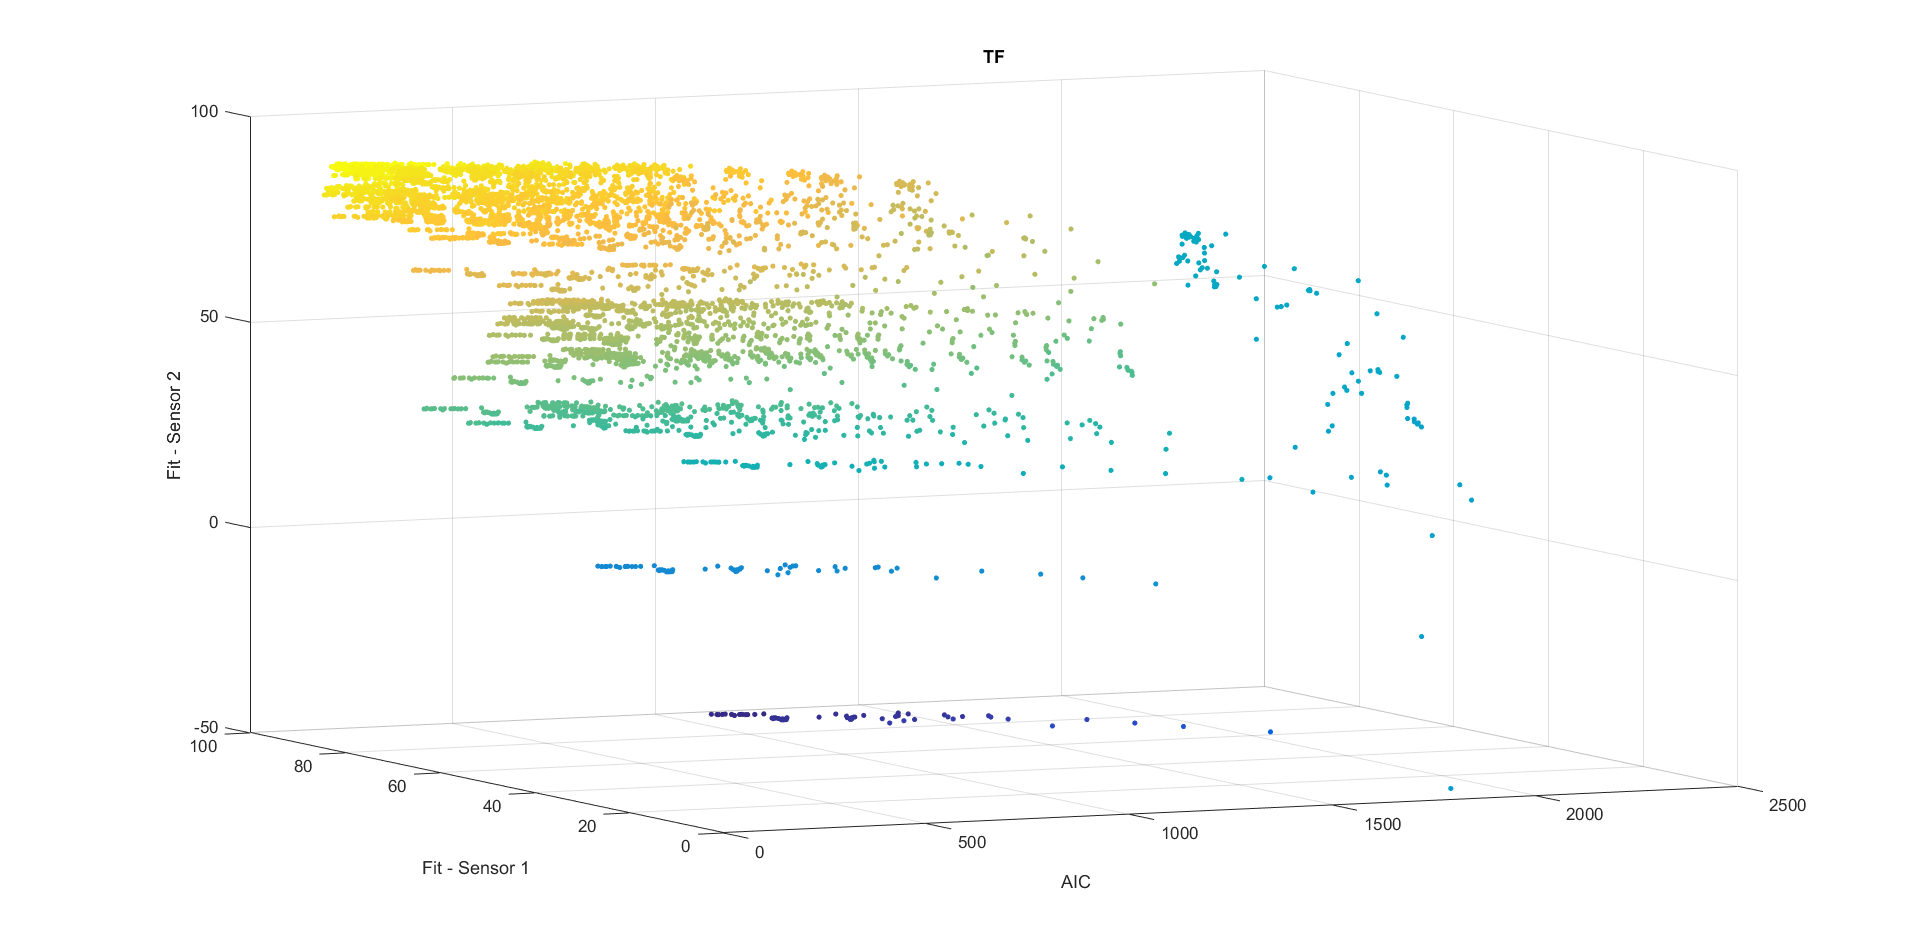
\includegraphics[width=1.00\textwidth]{./5_images/tclabsp-models-TF.png} 
		\label{fig:tclabsp-models-tf}
	\end{center}
	\centering
	\makebox[\width]{Fonte: Autor} 
\end{figure}

Cada um dos pontos presentes na \cref{fig:tclabsp-models-tf} representam um modelo experimental diferente, sendo que as cores
mais claras indicam aqueles com menor erro quando comparados ao conjunto de dados de validação.

A fim de escolher o melhor modelo de função de transferência frente aos 10000 gerados, os 10 primeiros modelos com menor 
valor segundo o critério de \acrshort{aic} foram submetidos à análise de resíduos (vide \cref{subsec:validacao_do_modelo}) e
dentre eles o que mostrou menor valor na análise resídual foi o modelo descrito na \cref{tab:tclabsp-model-tf}.
O teste deste modelo junto aos dados de validação e sua análise de resíduos podem ser visualizadas nas
\cref{fig:tclabsp-models-tf-compare,fig:tclabsp-models-tf-resid}, respectivamente.

\begin{table}[h]
	\centering
	\caption{Melhor modelo experimental - Função de transferência}
	\label{tab:tclabsp-model-tf}
	\begin{tabular}{c|c} \toprule
		{Entradas e saídas}		                                            & {Função de transferência}                                                                                                                                 \\ \midrule
        \begin{tabular}[c]{@{}l@{}}Aquecedor 1\\Sensor 1\end{tabular}		& $\frac{ 0.1248 z^{-1} - 0.01046 z^{-2} - 0.1142 z^{-3} }{ 1 - 0.8092 z^{-1} - 1.03 z^{-2} + 0.7405 z^{-3} + 0.1342 z^{-4} - 0.03503 z^{-5} }$             \\ \midrule
		\begin{tabular}[c]{@{}l@{}}Aquecedor 1\\Sensor 2\end{tabular}  		& $\frac{ 0.007869 z^{-1} - 0.007693 z^{-2} }{ 1 - 1.985 z^{-1} + 0.2452 z^{-2} + 1.659 z^{-3} - 1.083 z^{-4} + 0.1637 z^{-5} }$                            \\ \midrule
		\begin{tabular}[c]{@{}l@{}}Aquecedor 2\\Sensor 1\end{tabular}		& $\frac{ 0.00452 z^{-1}+ 0.005953 z^{-2} }{ 1 - 0.2164 z^{-1} - 1.301 z^{-2} + 0.2197 z^{-3} + 0.4412 z^{-4} - 0.08218 z^{-5} }$                           \\ \midrule
		\begin{tabular}[c]{@{}l@{}}Aquecedor 2\\Sensor 2\end{tabular}       & $\frac{ 0.06374 z^{-1} - 0.04266 z^{-2} }{ 1 - 1.504 z^{-1} + 0.4851 z^{-2} + 0.2172 z^{-3} - 0.2665 z^{-4} + 0.12 z^{-5} }$                              \\ \bottomrule
	\end{tabular}
	\caption*{Fonte: Autor}
\end{table}

% _____________________________________________________________________________________________________
% ___________________________________________ Paragraph _______________________________________________
% _____________________________________________________________________________________________________
\paragraph*{\textbf{Modelos experimentais de espaço de estados}}
\label{par:modelos_experimentais_ss}

Para a escolha do modelo experimental em espaço de estados foram testados 10 modelos de ordens distintas,
entre as ordens 1 e 10, e gráfico mostrando a comparação destes modelos frente ao critério de \acrshort{aic}
e aos dados de validação dos sensores 1 e 2 pode ser observado na \cref{fig:tclabsp-models-ss}.

Dentre todos os testados, o modelo de ordem 3 apresentou o menor valor no critério de \acrshort{aic} e foi
selecionado. O formato e as matrizes deste modelo podem ser vistos na \cref{eq:tclabsp-model-ss}
e o gráfico de teste junto aos dados de validação na \cref{fig:tclabsp-models-ss-compare}.

\begin{equation}
	\label{eq:tclabsp-model-ss}
	\begin{aligned}
		x(t + T_s) &= Ax(t) + Bu(t) + Ke(t)	\\
		y(t) &= Cx(t) + Du(t) + e(t)		\\
	\end{aligned}
\end{equation}

\begin{equation*}
	\begin{aligned}
		A &= \bbordermatrix{
											&	\textcolor{matrixtitle}{x_1}	&	\textcolor{matrixtitle}{x_2}	&	\textcolor{matrixtitle}{x_3}	\cr
			\textcolor{matrixtitle}{x_1}	&	0.9099							&	-0.02543						&	-0.02673	 					\cr
			\textcolor{matrixtitle}{x_2}	&	-0.06169						&	0.8193							&	-0.01098	 					\cr
			\textcolor{matrixtitle}{x_3}	&	-0.03506						&	0.108							&	0.9884		 					\cr
		}
		, \\
		C &= \bbordermatrix{
												&	\textcolor{matrixtitle}{x_1}	&	\textcolor{matrixtitle}{x_2}	&	\textcolor{matrixtitle}{x_3}	\cr
			\textcolor{matrixtitle}{Sensor_1}	&	180.1							&	8.69							&	1.814							\cr
			\textcolor{matrixtitle}{Sensor_2}	&	159.2							&	-40.71							&	1.665							\cr
		}
		,
	\end{aligned}
	\begin{aligned}
		B &= \bbordermatrix{
											&	\textcolor{matrixtitle}{Aquecedor_1}	&	\textcolor{matrixtitle}{Aquecedor_2}	\cr
			\textcolor{matrixtitle}{x_1}	&	0.0005512								&	7.033 \times 10^{-5}					\cr
			\textcolor{matrixtitle}{x_2}	&	0.002047								&	-0.001209								\cr
			\textcolor{matrixtitle}{x_3}	&	-0.0009257								&	0.0009081								\cr
		}
		, \\
		D &= \bbordermatrix{
												&	\textcolor{matrixtitle}{Aquecedor_1}	&	\textcolor{matrixtitle}{Aquecedor_2}	\cr
			\textcolor{matrixtitle}{Sensor_1}	&	0           							&	0										\cr
			\textcolor{matrixtitle}{Sensor_2}	&	0           							&	0										\cr
		}
		,
	\end{aligned}
\end{equation*}

\begin{equation*}
	K = \bbordermatrix{
										&	\textcolor{matrixtitle}{Sensor_1}	&	\textcolor{matrixtitle}{Sensor_2}	\cr
		\textcolor{matrixtitle}{x_1}	&	0.000946							&	0.0008267							\cr
		\textcolor{matrixtitle}{x_2}	&	0.0006276							&	0.001956							\cr
		\textcolor{matrixtitle}{x_3}	&	-0.008009							&	0.003641							\cr
	}
\end{equation*}

% _____________________________________________________________________________________________________
% ___________________________________________ Paragraph _______________________________________________
% _____________________________________________________________________________________________________
\paragraph*{\textbf{Modelos experimentais ARX}}
\label{par:modelos_experimentais_arx}

Os modelos \acrshort{arx} foram criados a partir de combinações de diferentes números de pólos ($n_a$),
números de zeros ($n_b$) e de tempo morto ($n_k$). As combinações utilizadas podem ser vistas na
\cref{tab:tclabsp-models-arx}.

\begin{table}[h]
	\centering
	\caption{Modelos experimentais - ARX}
	\label{tab:tclabsp-models-arx}
	\begin{tabular}{c|c} \toprule
		{Parâmetro}		&	{Valores utilizados nas combinações}									\\ \midrule
		$n_a$			&
							$ \begin{bmatrix}	1	&	1	\\	1	&	1	\\	\end{bmatrix} $	,		
							$ \begin{bmatrix}	2	&	2	\\	2	&	2	\\	\end{bmatrix} $	,		
							$ \begin{bmatrix}	3	&	3	\\	3	&	3	\\	\end{bmatrix} $	,		
							$ \begin{bmatrix}	4	&	4	\\	4	&	4	\\	\end{bmatrix} $		\\ \midrule
		$n_b$			&
							$ \begin{bmatrix}	1	&	1	\\	1	&	1	\\	\end{bmatrix} $	,		
							$ \begin{bmatrix}	2	&	2	\\	2	&	2	\\	\end{bmatrix} $	,		
							$ \begin{bmatrix}	3	&	3	\\	3	&	3	\\	\end{bmatrix} $	 	\\ \midrule
		$n_k$			&
							$ \begin{bmatrix}	1	&	1	\\	1	&	1	\\	\end{bmatrix} $		\\ \bottomrule
	\end{tabular}
	\caption*{Fonte: Autor}
\end{table}

O gráfico mostrando a distribuição dos modelos gerados em comparação ao critério de \acrshort{aic} pode ser
visto na \cref{fig:tclabsp-models-arx} e o modelo \acrshort{arx} escolhido, seu gráfico comparativo aos dados validação
e sua análise residual podem ser vistos na \cref{tab:tclabsp-model-arx}, na \cref{fig:tclabsp-models-arx-compare} e na
\cref{fig:tclabsp-models-arx-resid}, respectivamente.

\begin{table}[h]
	\centering
	\caption{Melhor modelo experimental - ARX}
	\label{tab:tclabsp-model-arx}
	\begin{tabular}{c|c} \toprule
		{Saída}			&	{Parâmetros}									\\ \midrule
		$Sensor_1$			&
								$ 
									\begin{aligned}
										\text{Formato:}																	\\
										A(z)y_1(t) &= - A_i(z)y_i(t) + B(z)u(t) + e_1(t)								\\
										\text{Onde:}																	\\
										A(z) &= 1 - 1.308 z^{-1} + 0.1507 z^{-2} + 0.3109 z^{-3} - 0.07434 z^{-4}       \\  
										A_2(z) &= -0.2768 z^{-1} + 0.03432 z^{-2} + 0.1842 z^{-3} - 0.02748 z^{-4}      \\  
										B1(z) &= 0.07487 z^{-1} - 0.02 z^{-2} - 0.01542 z^{-3}                      	\\
										B2(z) &= -0.00504 z^{-1} - 0.006801 z^{-2} - 0.01316 z^{-3}    
									\end{aligned}
								$	
							\\ \midrule
		$Sensor_2$			&
								$ 
									\begin{aligned}
										\text{Formato:}																	\\
										A(z)y_2(t) &= - A_i(z)y_i(t) + B(z)u(t) + e_2(t)								\\
										\text{Onde:}																	\\
										A(z) &= 1 - 0.4098 z^{-1} - 0.2493 z^{-2} + 0.0703 z^{-3} - 0.1442 z^{-4}    	\\   
										A_1(z) &= -0.9008 z^{-1} + 0.257 z^{-2} + 0.5452 z^{-3} - 0.1428 z^{-4}  		\\
										B1(z) &= -0.02857 z^{-1} - 0.06333 z^{-2} - 0.03838 z^{-3}          			\\
										B2(z) &= 0.05223 z^{-1} + 0.025 z^{-2} + 0.01699 z^{-3} 		
									\end{aligned}
								$
							\\ \bottomrule
	\end{tabular}
	\caption*{Fonte: Autor}
\end{table}

% _____________________________________________________________________________________________________
% ___________________________________________ Paragraph _______________________________________________
% _____________________________________________________________________________________________________
\paragraph*{\textbf{Modelos experimentais ARMAX}}
\label{par:modelos_experimentais_armax}

De forma análoga ao procedimento realizado para a obtenção dos modelos \acrshort{arx}, os modelos
\acrshort{armax} também foram criados a partir de combinações de diferentes números de pólos ($n_a$),
números de zeros mais 1 ($n_b$), número de coeficientes C ($n_c$) e de tempo morto ($n_k$).
As combinações utilizadas podem ser vistas na \cref{tab:tclabsp-models-armax}.

\begin{table}[h]
	\centering
	\caption{Modelos experimentais - ARMAX}
	\label{tab:tclabsp-models-armax}
	\begin{tabular}{c|c} \toprule
		{Parâmetro}		&	{Valores utilizados nas combinações}									\\ \midrule
		$n_a$			&
							$ \begin{bmatrix}	1	&	1	\\	1	&	1	\\	\end{bmatrix} $	,		
							$ \begin{bmatrix}	2	&	2	\\	2	&	2	\\	\end{bmatrix} $	,		
							$ \begin{bmatrix}	3	&	3	\\	3	&	3	\\	\end{bmatrix} $	,		
							$ \begin{bmatrix}	4	&	4	\\	4	&	4	\\	\end{bmatrix} $		\\ \midrule
		$n_b$			&
							$ \begin{bmatrix}	1	&	1	\\	1	&	1	\\	\end{bmatrix} $	,		
							$ \begin{bmatrix}	2	&	2	\\	2	&	2	\\	\end{bmatrix} $	,		
							$ \begin{bmatrix}	3	&	3	\\	3	&	3	\\	\end{bmatrix} $		\\ \midrule
		$n_c$			&
							$ \begin{bmatrix}	1	&	1	\\	1	&	1	\\	\end{bmatrix} $	,		
							$ \begin{bmatrix}	2	&	2	\\	2	&	2	\\	\end{bmatrix} $	,		
							$ \begin{bmatrix}	3	&	3	\\	3	&	3	\\	\end{bmatrix} $	,		
							$ \begin{bmatrix}	4	&	4	\\	4	&	4	\\	\end{bmatrix} $		\\ \midrule
		$n_k$			&
							$ \begin{bmatrix}	1	&	1	\\	1	&	1	\\	\end{bmatrix} $		\\ \bottomrule
	\end{tabular}
	\caption*{Fonte: Autor}
\end{table}

A partir de todos os modelos possíveis gerados a partir das combinações dos parâmetros da \cref{tab:tclabsp-models-armax},
selecionaram-se os 10 modelos com menor valor segundo o critério de \acrshort{aic} e a partir destes foi então
selecionado o modelo com menor valor residual.
O gráfico mostrando a distribuição dos modelos gerados em comparação ao critério de \acrshort{aic} pode ser
visto na \cref{fig:tclabsp-models-armax} e o modelo \acrshort{armax} escolhido, seu gráfico comparativo aos dados validação
e sua análise residual podem ser vistos na \cref{tab:tclabsp-model-armax}, na \cref{fig:tclabsp-models-armax-compare} e na
\cref{fig:tclabsp-models-armax-resid}, respectivamente.

\begin{table}[h]
	\centering
	\caption{Melhor modelo experimental - ARMAX}
	\label{tab:tclabsp-model-armax}
	\begin{tabular}{c|c} \toprule
		{Saída}			&	{Parâmetros}									\\ \midrule
		$Sensor_1$			&
								$ 
									\begin{aligned}
										\text{Formato:}													\\
										A(z)y_1(t) &= - A_i(z)y_i(t) + B(z)u(t) + C(z)e_1(t)			\\
										\text{Onde:}													\\
										A(z) &= 1 - 1.804 z^{-1} + 0.8137 z^{-2}      					\\
										A_2(z) &= -0.09524 z^{-1} + 0.08503 z^{-2}  					\\							
										B1(z) &= 0.1164 z^{-1} - 0.1108 z^{-2}     						\\				
										B2(z) &= 0.004773 z^{-1} - 0.008481 z^{-2} 						\\				
										C(z) &= 1 - 1.683 z^{-1} + 0.6901 z^{-2}    
									\end{aligned}
								$	
							\\ \midrule
		$Sensor_2$			&
								$ 
									\begin{aligned}
										\text{Formato:}													\\
										A(z)y_2(t) &= - A_i(z)y_i(t) + B(z)u(t) + C(z)e_2(t)			\\
										\text{Onde:}													\\
										A(z) &= 1 - 1.72 z^{-1} + 0.7437 z^{-2}       					\\
										A_1(z) &= -0.1496 z^{-1} + 0.1278 z^{-2}   						\\				
										B1(z) &= 0.003022 z^{-1} - 0.01553 z^{-2} 						\\				
										B2(z) &= 0.06256 z^{-1} - 0.05434 z^{-2}  						\\				
										C(z) &= 1 - 1.67 z^{-1} + 0.6744 z^{-2}     			
									\end{aligned}
								$
							\\ \bottomrule
	\end{tabular}
	\caption*{Fonte: Autor}
\end{table}

% _____________________________________________________________________________________________________
% ___________________________________________ Paragraph _______________________________________________
% _____________________________________________________________________________________________________
\paragraph*{\textbf{Modelos experimentais OE}}
\label{par:modelos_experimentais_oe}

Os modelos \acrshort{oe} foram criados a partir de combinações de diferentes ordens do polinômio B+1 ($n_b$),
ordens do polinômio F ($n_f$) e de tempo morto ($n_k$). As combinações utilizadas podem ser vistas na
\cref{tab:tclabsp-models-oe}.

\begin{table}[h]
	\centering
	\caption{Modelos experimentais - OE}
	\label{tab:tclabsp-models-oe}
	\begin{tabular}{c|c} \toprule
		{Parâmetro}		&	{Valores utilizados nas combinações}									\\ \midrule
		$n_b$			&
							$ \begin{bmatrix}	1	&	1	\\	1	&	1	\\	\end{bmatrix} $	,		
							$ \begin{bmatrix}	2	&	2	\\	2	&	2	\\	\end{bmatrix} $	,		
							$ \begin{bmatrix}	3	&	3	\\	3	&	3	\\	\end{bmatrix} $	,		
							$ \begin{bmatrix}	4	&	4	\\	4	&	4	\\	\end{bmatrix} $		\\ \midrule
		$n_f$			&
							$ \begin{bmatrix}	1	&	1	\\	1	&	1	\\	\end{bmatrix} $	,		
							$ \begin{bmatrix}	2	&	2	\\	2	&	2	\\	\end{bmatrix} $	,		
							$ \begin{bmatrix}	3	&	3	\\	3	&	3	\\	\end{bmatrix} $	,		
							$ \begin{bmatrix}	4	&	4	\\	4	&	4	\\	\end{bmatrix} $		\\ \midrule
		$n_k$			&
							$ \begin{bmatrix}	1	&	1	\\	1	&	1	\\	\end{bmatrix} $		\\ \bottomrule
	\end{tabular}
	\caption*{Fonte: Autor}
\end{table}

A partir de todos os modelos gerados a partir das combinações dos parâmetros da \cref{tab:tclabsp-models-oe},
ordenaram-se os modelos com menor valor segundo o critério de \acrshort{aic} e a partir destes foi então
selecionado o modelo com menor valor residual.
O gráfico mostrando a distribuição dos modelos gerados em comparação ao critério de \acrshort{aic} pode ser
visto na \cref{fig:tclabsp-models-oe} e o modelo \acrshort{oe} escolhido, seu gráfico comparativo aos dados validação
e sua análise residual podem ser vistos na \cref{tab:tclabsp-model-oe}, na \cref{fig:tclabsp-models-oe-compare} e na
\cref{fig:tclabsp-models-oe-resid}, respectivamente.

\begin{table}[h]
	\centering
	\caption{Melhor modelo experimental - OE}
	\label{tab:tclabsp-model-oe}
	\begin{tabular}{c|c} \toprule
		{Saída}			&	{Parâmetros}									\\ \midrule
		$Sensor_1$			&
								$ 
									\begin{aligned}
										\text{Formato:}														\\
										y_1(t) &= \frac{B(z)}{F(z)}u(t) + e_1(t)							\\
										\text{Onde:}														\\
										B1(z) &= 0.08894 z^{-1} + 0.04175 z^{-2} - 0.09187 z^{-3}   		\\
										B2(z) &= 0.008258 z^{-1} + 0.001846 z^{-2} - 0.01011 z^{-3} 		\\
										F1(z) &= 1 - 0.912 z^{-1} - 0.5633 z^{-2} + 0.5215 z^{-3}  			\\
										F2(z) &= 1 - 0.9537 z^{-1} - 0.9783 z^{-2} + 0.932 z^{-3}    
									\end{aligned}
								$	
							\\ \midrule
		$Sensor_2$			&
								$ 
									\begin{aligned}
										\text{Formato:}														\\
										y_2(t) &= \frac{B(z)}{F(z)}u(t) + e_2(t)							\\
										\text{Onde:}														\\
										B1(z) &= -0.005385 z^{-1} + 0.02174 z^{-2} - 0.01629 z^{-3}    		\\
										B2(z) &= 0.06252 z^{-1} - 0.08437 z^{-2} + 0.0602 z^{-3}			\\
										F1(z) &= 1 - 2.394 z^{-1} + 1.824 z^{-2} - 0.4304 z^{-3} 			\\
										F2(z) &= 1 - 2.217 z^{-1} + 2.138 z^{-2} - 0.8374 z^{-3}  	
									\end{aligned}
								$
							\\ \bottomrule
	\end{tabular}
	\caption*{Fonte: Autor}
\end{table}

% _____________________________________________________________________________________________________
% ___________________________________________ Paragraph _______________________________________________
% _____________________________________________________________________________________________________
\paragraph*{\textbf{Modelos experimentais Box-Jenkins}}
\label{par:modelos_experimentais_bj}

Os modelos \acrshort{bj} foram criados a partir de combinações de diferentes ordens do polinômio B+1 ($n_b$),
ordens do polinômio C+1 ($n_c$), ordens do polinômio D+1 ($n_d$), ordens do polinômio F+1 ($n_f$)
e do tempo morto ($n_k$). As combinações utilizadas podem ser vistas na
\cref{tab:tclabsp-models-bj}.

\begin{table}[h]
	\centering
	\caption{Modelos experimentais - BJ}
	\label{tab:tclabsp-models-bj}
	\begin{tabular}{c|c} \toprule
		{Parâmetro}		&	{Valores utilizados nas combinações}									\\ \midrule
		$n_b$			&
							$ \begin{bmatrix}	1	&	1	\\	1	&	1	\\	\end{bmatrix} $	,		
							$ \begin{bmatrix}	2	&	2	\\	2	&	2	\\	\end{bmatrix} $	,		
							$ \begin{bmatrix}	3	&	3	\\	3	&	3	\\	\end{bmatrix} $	,		
							$ \begin{bmatrix}	4	&	4	\\	4	&	4	\\	\end{bmatrix} $		\\ \midrule
		$n_c$			&
							$ \begin{bmatrix}	1	&	1	\\	1	&	1	\\	\end{bmatrix} $	,		
							$ \begin{bmatrix}	2	&	2	\\	2	&	2	\\	\end{bmatrix} $	,		
							$ \begin{bmatrix}	3	&	3	\\	3	&	3	\\	\end{bmatrix} $	,		
							$ \begin{bmatrix}	4	&	4	\\	4	&	4	\\	\end{bmatrix} $		\\ \midrule
		$n_d$			&
							$ \begin{bmatrix}	1	&	1	\\	1	&	1	\\	\end{bmatrix} $	,		
							$ \begin{bmatrix}	2	&	2	\\	2	&	2	\\	\end{bmatrix} $	,		
							$ \begin{bmatrix}	3	&	3	\\	3	&	3	\\	\end{bmatrix} $	,		
							$ \begin{bmatrix}	4	&	4	\\	4	&	4	\\	\end{bmatrix} $		\\ \midrule
		$n_f$			&
							$ \begin{bmatrix}	1	&	1	\\	1	&	1	\\	\end{bmatrix} $	,		
							$ \begin{bmatrix}	2	&	2	\\	2	&	2	\\	\end{bmatrix} $	,		
							$ \begin{bmatrix}	3	&	3	\\	3	&	3	\\	\end{bmatrix} $	,		
							$ \begin{bmatrix}	4	&	4	\\	4	&	4	\\	\end{bmatrix} $		\\ \midrule
		$n_k$			&
							$ \begin{bmatrix}	1	&	1	\\	1	&	1	\\	\end{bmatrix} $		\\ \bottomrule
	\end{tabular}
	\caption*{Fonte: Autor}
\end{table}

A partir de todos os modelos possíveis gerados a partir das combinações dos parâmetros da \cref{tab:tclabsp-models-bj},
selecionaram-se os 10 modelos com menor valor segundo o critério de \acrshort{aic} e a partir destes foi então
selecionado o modelo com menor valor residual.
O gráfico mostrando a distribuição dos modelos gerados em comparação ao critério de \acrshort{aic} pode ser
visto na \cref{fig:tclabsp-models-bj} e o modelo \acrshort{bj} escolhido, seu gráfico comparativo aos dados validação
e sua análise residual podem ser vistos na \cref{tab:tclabsp-model-bj}, na \cref{fig:tclabsp-models-bj-compare} e na
\cref{fig:tclabsp-models-bj-resid}, respectivamente.

\begin{table}[h]
	\centering
	\caption{Melhor modelo experimental - BJ}
	\label{tab:tclabsp-model-bj}
	\begin{tabular}{c|c} \toprule
		{Saída}			&	{Parâmetros}									\\ \midrule
		$Sensor_1$			&
								$ 
									\begin{aligned}
										\text{Formato:}														\\
										y_1(t) &= \frac{B(z)}{F(z)}u(t) + \frac{C(z)}{D(z)}e_1(t)			\\
										\text{Onde:}														\\
										B1(z) &= 0.1123 z^{-1} - 0.07415 z^{-2} 							\\
										B2(z) &= 0.007474 z^{-1} - 0.005786 z^{-2}  						\\		
										C(z) &= 1 - 0.7216 z^{-1} - 0.1974 z^{-2}  							\\	
										D(z) &= 1 - z^{-1}  												\\	
										F1(z) &= 1 - 1.531 z^{-1} + 0.5793 z^{-2}  							\\	
										F2(z) &= 1 - 1.866 z^{-1} + 0.8761 z^{-2}  
									\end{aligned}
								$	
							\\ \midrule
		$Sensor_2$			&
								$ 
									\begin{aligned}
										\text{Formato:}														\\
										y_2(t) &= \frac{B(z)}{F(z)}u(t) + \frac{C(z)}{D(z)}e_2(t)			\\
										\text{Onde:}														\\
										B1(z) &= 0.00393 z^{-1} + 0.001759 z^{-2} 							\\
										B2(z) &= 0.06455 z^{-1} - 0.02444 z^{-2}  							\\	
										C(z) &= 1 - 0.8508 z^{-1} - 0.09047 z^{-2} 							\\	
										D(z) &= 1 - z^{-1}  												\\	
										F1(z) &= 1 - 1.678 z^{-1} + 0.6984 z^{-2} 							\\	
										F2(z) &= 1 - 1.218 z^{-1} + 0.3003 z^{-2}    			
									\end{aligned}
								$
							\\ \bottomrule
	\end{tabular}
	\caption*{Fonte: Autor}
\end{table}

% -----------------------------------------------------------------------------------------------------
% ------------------------------------------- Subsubsection -------------------------------------------
% -----------------------------------------------------------------------------------------------------
\subsection{Comparativo}
\label{subsec:modelos_experimentais_comparativo}

Comparando todos os modelos experimentais escolhidos nos diferentes formatos é possível verificar que,
apesar de grandes diferenças estruturais em comparação ao modelo teórico da \cref{eq:tclab_modelo_teorico}, os
modelos experimentais apresentaram em geral resultados satisfatórios quando submetidos a testes de validação,
com exceção apenas do modelo \acrshort{arx} que teve um desempenho médio aproximadamente $30\%$ inferior
aos demais modelos avaliados.
Um gráfico comparativo com todos os modelos experimentais escolhidos pode ser observado na 
\cref{fig:comparativo_modelos_experimentais} e na \cref{tab:modelos_experimentais_fit} é apresentada uma
consolidação dos valores de aproximação aos dados de validação para cada um dos modelos. 

\begin{figure}[h]
	\caption{Comparativo dos modelos experimentais}
	\begin{center}
		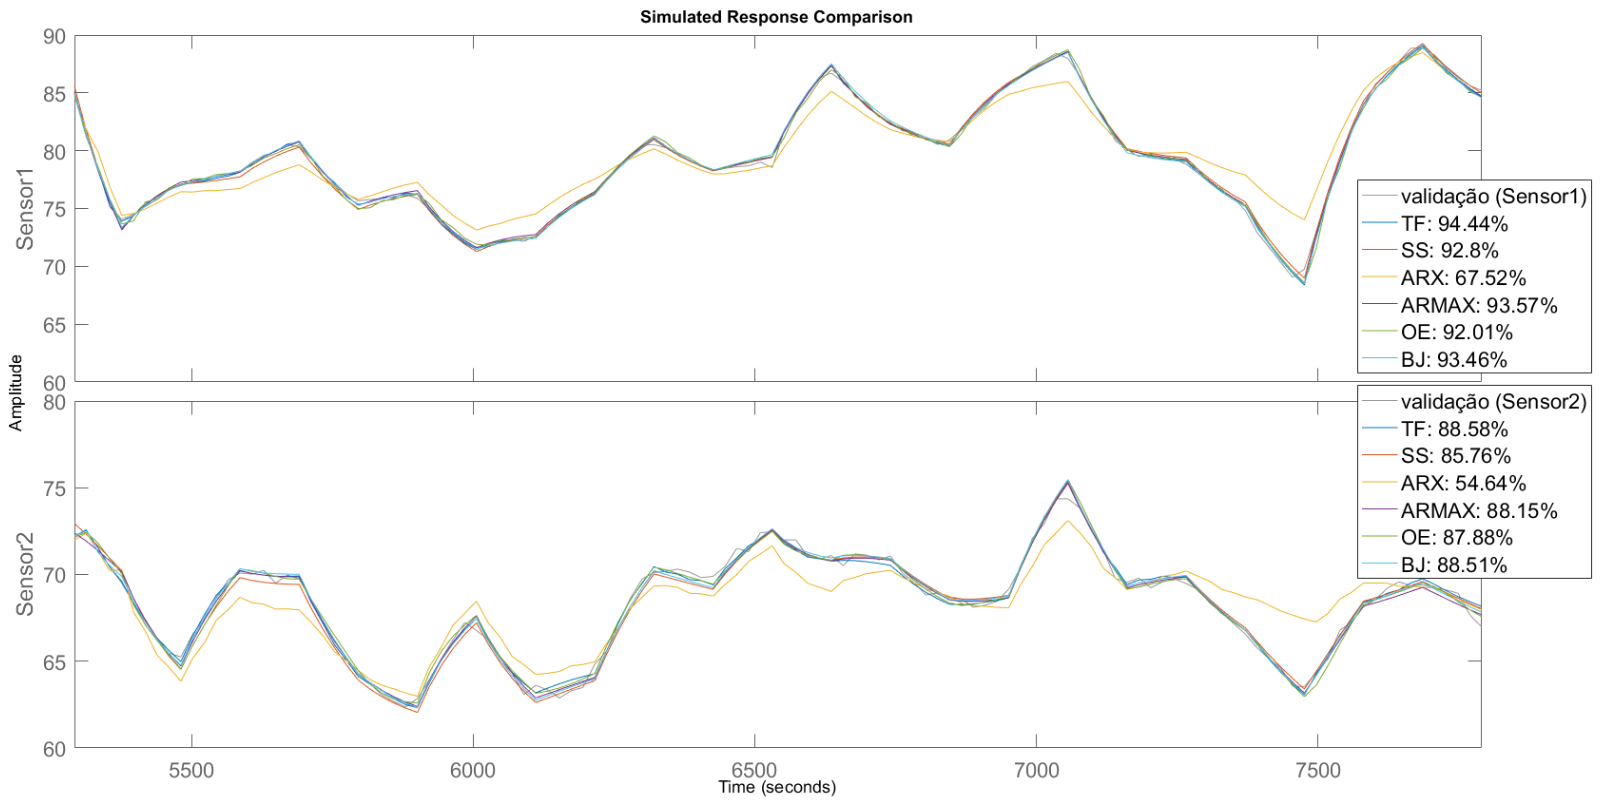
\includegraphics[width=1.00\textwidth]{./5_images/tclabsp-models-ALL-compare.png} 
		\label{fig:comparativo_modelos_experimentais}
	\end{center}
	\centering
	\makebox[\width]{Fonte: Autor} 
\end{figure}

\begin{table}[h]
	\centering
	\caption{Qualidade dos modelos experimentais}
	\label{tab:modelos_experimentais_fit}
	\begin{tabular}{c|cc} \toprule
		{Modelo}		                            			&	{\textit{Fit} Sensor 1}	    &	{\textit{Fit} Sensor 2}			\\ \midrule
		\acrshort{tf} (\cref{tab:tclabsp-model-tf})				&   $94.44\%$                   &   $88.58\%$                       \\
		\acrshort{bj} (\cref{tab:tclabsp-model-bj})				&   $93.46\%$                   &   $88.51\%$                       \\ 
		\acrshort{armax} (\cref{tab:tclabsp-model-armax})		&   $93.57\%$                   &   $88.15\%$                       \\
		\acrshort{oe} (\cref{tab:tclabsp-model-oe})				&   $92.01\%$                   &   $87.88\%$                       \\
		\acrshort{ss} (\cref{eq:tclabsp-model-ss})			    &   $92.80\%$                   &   $85.76\%$                       \\
		\acrshort{arx}	(\cref{tab:tclabsp-model-arx})		    &   $67.52\%$                   &   $54.64\%$                       \\ \bottomrule
	\end{tabular}
	\caption*{Fonte: Autor}
\end{table}

\chapter{Desenvolvimento do controlador}
\label{ch:desenvolvimento_controlador}

Com o intuito de controlar o \acrshort{tclabsp} aplicando o \acrshort{mpc} como técnica,
utilizaram-se os modelos teóricos e experimentais apresentados na \cref{sec:modelagem_da_planta_piloto}
e na \cref{sec:modelo_experimental} para o desenvolvimento do bloco controlador no \textit{Simulink}.
Um controlador \acrshort{pid} também foi desenvolvido a fim de servir como base comparativa ao
controlador \acrshort{mpc} criado.
A seção a seguir descreve este controlador \acrshort{pid}.

% =====================================================================================================
% ============================================= Section ===============================================
% =====================================================================================================
\section{Controlador PID}
\label{sec:controlador_pid}

O controlador \acrshort{pid} desenvolvido foi criado em ambiente \textit{Simulink},
utilizando o aplicativo \textit{PID Tuner} do \acrshort{matlab}, disponível através do pacote
\textit{Control System Toolbox}.

A cada um dos Aquecedores do \acrshort{tclabsp} foi conectado a um bloco \textit{PID Controller} retroalimentado
com a saída dos Sensores de Temperatura da planta, conforme ilustrado pela \cref{fig:pidcreation}.

\begin{figure}[h]
	\caption{Modelo Simulink do controlador PID}
	\begin{center}
		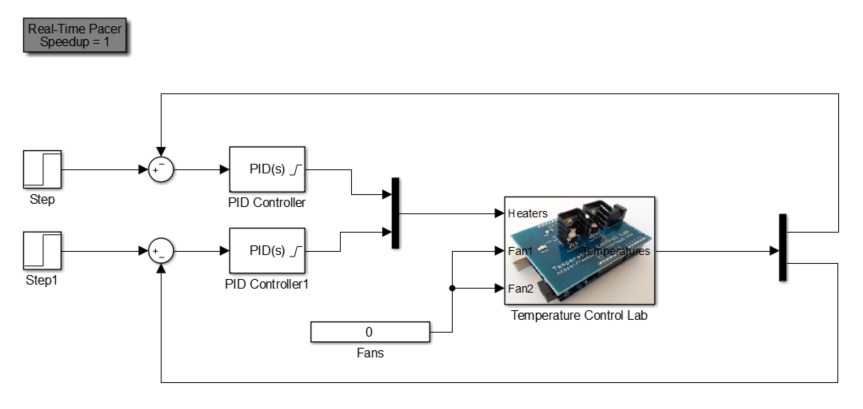
\includegraphics[width=1.00\textwidth]{./5_images/PIDCreation.png} 
		\label{fig:pidcreation}
	\end{center}
	\centering
	\makebox[\width]{Fonte: Autor} 
\end{figure}

Os blocos \textit{PID Controller} foram inicialmente configurados com os limites de saturação de saída
entre 0 e 100 para que nenhum valor fora desta faixa fosse aplicado a planta controlada.
Em seguida, uma vez que o desenvolvimento do controlador \acrshort{pid} não era um objetivo deste trabalho,
utilizou-se a função de auto-sintonia do \textit{PID Tuner} para encontrar valores satisfatórios de controle
do sistema.

A \cref{tab:pid_values} apresenta os valores de sintonia encontrados para um controlador \acrshort{pid}
paralelo (\cref{eq:pid_format}).

\begin{equation}
    \label{eq:pid_format}
    P + I \frac{1}{s} + D \frac{N}{1 + N \frac{1}{s}}
\end{equation}

\begin{table}[h]
	\centering
	\caption{Sintonia dos blocos PID}
	\label{tab:pid_values}
	\begin{tabular}{c|cc} \toprule
		{Parâmetro}		            & {PID Aquecedor 1}     & {PID Aquecedor 2}           \\ \midrule
		Proporcional (P)		    & $1.435$               & $2.182$                     \\
		Integral (I)   		        & $0.016$               & $0.011$                     \\
		Derivativo (D)		        & $-9.119$              & $-30.919$                   \\
		Filtro (N)                  & $0.0216$              & $0.010$                     \\ \bottomrule
	\end{tabular}
	\caption*{Fonte: Autor}
\end{table}


% =====================================================================================================
% ============================================= Section ===============================================
% =====================================================================================================
\section{Controlador MPC}
\label{sec:controlador_mpc}

Segundo \citeonline{Alhajeri2020}, o grande número de parâmetros sintonizáveis motivou diversos estudos
sobre como sintonizar o \acrshort{mpc} e nesta seção serão indicadas as técnicas utilizadas na sintonia de cada
um dos parâmetros do controle \acrshort{mpc} em questão.

% .....................................................................................................
% ............................................ Subsection .............................................
% .....................................................................................................
\subsection{Horizonte de predição}
\label{subsec:horizonte_de_predicao}

A janela de tempo que especifica quantos períodos de amostragem futuros sobre os quais a resposta da 
variável controlada $y_i$ será predita pelo modelo da planta e então otimizada é chamado de horizonte
de predição \cite{Alhajeri2020}. Este horizonte é indicado pela letra $P$ e seus limites inferiores
e superiores são, respectivamente, $P_{0_{n_y}}$ e $P_{n_y}$. Importante notar que o horizonte de predição
é calculado para cada saída $n_y$, portanto em um sistema com 2 saídas, por exemplo, os limites inferiores
serão $P_{0_1}$ e $P_{0_2}$ e os limites superiores $P_1$ e $P_2$.

No seu estudo sobre as diferentes técnicas de sintonia do \acrshort{mpc}, \citeonline{Alhajeri2020} indicam
que, no geral, o horizonte de predição deve ser adequadamente grande para que as predições das saídas
controladas possam representar uma porção significativa do processo, portanto valores altos devem
ser selecionados para $P_1$, $\cdots$, $P_{n_y}$, para assegurar a estabilidade e robustez em malha fechada.
Contudo, quanto maiores forem estes valores, maior será o custo computacional para a resolução do
problema de otimização do \acrshort{mpc}. Na prática, aumentar os valores de $P_1$, $\cdots$, $P_{n_y}$
aumenta a robustez e a estabilidade, porém após certos valores o aumento desta janela de predição não
altera a performance de controle significativamente, mas irá intensificar a carga computacional, o que
pode deteriorar a robustez do controle.

As \cref{eq:horizonte_de_predicao_lim_inf_no_delay,eq:horizonte_de_predicao_lim_inf_with_delay},
sugeridas por \citeonline{Alhajeri2020}, indicam os valores de limite inferior do horizonte de predição
 para plantas sem atraso e com atraso, respectivamente.

\begin{equation}
	\label{eq:horizonte_de_predicao_lim_inf_no_delay}
    P_{0_1} = 1, \cdots, P_{0_{n_y}} = 1
\end{equation}

\begin{equation}
	\label{eq:horizonte_de_predicao_lim_inf_with_delay}
	P_{0_1} = 1 + \frac{\min_j \left( \sum_{j=1}^{n_u} \theta_{1_j} \right)}{t_s}		\\
	, \cdots,																			\\
	P_{0_{n_y}} = 1 + \frac{\min_j \left( \sum_{j=1}^{n_u} \theta_{{n_y}_j} \right)}{t_s}
\end{equation}

\noindent
Onde: 
\begin{itemize}
	\item $n_u$: são as entradas do sistema
	\item $\theta_i$: é o tempo morto da planta
	\item $t_s$: é o período de amostragem
\end{itemize}

Os mesmos autores indicam estudos que sugerem que o limite superior seja calculados segundo
as \cref{eq:horizonte_de_predicao_lim_sup_no_delay,eq:horizonte_de_predicao_lim_sup_with_delay},
sendo a primeira sem a utilização de tempo morto, e a segunda, considerando o tempo morto da planta.

\begin{equation}
	\label{eq:horizonte_de_predicao_lim_sup_no_delay}
    P_{1} = \frac{0.8 * T_s}{t_s} , \cdots, P_{{n_y}} = \frac{0.8 * T_s}{t_s}
\end{equation}

\begin{equation}
	\label{eq:horizonte_de_predicao_lim_sup_with_delay}
	\begin{aligned}
		\frac{\max_j \left( \sum_{j=1}^{n_u} \theta_{1_j} \right)}{t_s} + 1					
		\leqslant P_1 \leqslant																
		\frac{\max_j \left( \sum_{j=1}^{n_u} \theta_{1_j} \right)}{t_s} + 					
		\max_J \left( \sum_{j=1}^{n_u} M_j \right)											
		, \cdots,																			\\
		\frac{\max_j \left( \sum_{j=1}^{n_u} \theta_{{n_y}_j} \right)}{t_s} + 1				
		\leqslant P_{n_y} \leqslant															
		\frac{\max_j \left( \sum_{j=1}^{n_u} \theta_{{n_y}_j} \right)}{t_s} + 				
		\max_J \left( \sum_{j=1}^{n_u} M_j \right)
	\end{aligned}
\end{equation}

\noindent
Onde: 
\begin{itemize}
	\item $n_u$: são as entradas do sistema
	\item $\theta_i$: é o tempo morto da planta
	\item $t_s$: é o período de amostragem
	\item $T_s$: é o maior tempo de acomodação das variáveis controladas em malha aberta
	\item $M_i$: é o horizonte de controle 
\end{itemize}

% .....................................................................................................
% ............................................ Subsection .............................................
% .....................................................................................................
\subsection{Horizonte de controle}
\label{subsec:horizonte_de_controle}

O horizonte de controle, representado por $M_i$, são os valores da variável manipulada que o controlador
calcula a cada instante de tempo, ou seja, $u_i(k), \cdots, u_i(k+M_i-1)$. O incremento deste horizonte
aumenta também a agressividade, a habilidade para estabilizar plantas instáveis e o custo computacional,
porém diminui a robustez do sistema de controle \cite{Alhajeri2020}.

Segundo o levantamento de \citeonline{Alhajeri2020}, diferentes estudos apontaram que o ajuste recomendado
para o horizonte de controle seria o indicado na \cref{eq:horizonte_de_controle}, pois não foi observada
nenhuma melhoria expressiva da performance do controle em malha fechada com valores superiores a este.

\begin{equation}
	\label{eq:horizonte_de_controle}
	\begin{aligned}
		M_i \leqslant 2,			\\
		i = 1, \cdots, n_u
	\end{aligned}
\end{equation}

% .....................................................................................................
% ............................................ Subsection .............................................
% .....................................................................................................
\subsection{Matrizes de peso}
\label{subsec:matrizes_de_peso}

Além dos horizontes de predição e de controle, as matrizes de peso $Q$, $R$ e $\Delta$ também são parâmetros
que necessitam ser ajustados para aprimorar a sintonia do controlador \acrshort{mpc}.

A matriz $Q$ configura a penalidade nos erros das saídas. Os elementos dessa matriz penalizam o desvio 
das saídas em comparação a suas trajetórias de referência. Eles refletem o custo relativo das variáveis 
controladas desviando de suas trajetórias de referência e, portanto, dos seus \textit{set-points}
\cite{Alhajeri2020}.

As matrizes $R$ e $\Delta$ descrevem a penalidade na taxa de variação das entradas e na magnitude das mesmas, 
respectivamente. O valor relativo dos elementos de $\Delta$ são um indicativo do custo relativo das 
entradas manipuladas \cite{Alhajeri2020}.

Segundo \citeonline{Alhajeri2020}, normalmente assume-se que $\Delta = 0$, a menos que uma diretriz de 
sintonia diferente seja mencionada. Já para as matrizes $Q$ e $R$, muitos estudos indicam que
$Q = I$ e $R = \rho I$, onde $\rho$ é um escalar também conhecido como \textit{fator de supressão de movimento}.
Esta abordagem, de encontrar um valor para $\rho$ ao invés de encontrar as matrizes de peso, ao mesmo tempo que
simplifica a tarefa de sintonizar o controlador \acrshort{mpc}, retira certa flexibilidade do controle e
limita o grau de qualidade que o \acrshort{mpc} pode prover.

Um dos estudos apresentados por \citeonline{Alhajeri2020} sugere a utilização de $\rho = 0.01$ para um controle
\acrshort{mpc} sem restrições e $\rho = 0.1$ para um controle com restrições. Dessa forma as matrizes utilizadas
neste tralhado são indicadas na \cref{eq:matrizes_de_peso}.

\begin{equation}
	\label{eq:matrizes_de_peso}
	\begin{aligned}
		\Delta &= 0																\\
		Q &= I																	\\
		R &= \rho I,															\\
		\text{sendo: } \rho &= 0.01 \text{ (\acrshort{mpc} sem restrições)}		\\
		\rho &= 0.1 \text{ (\acrshort{mpc} com restrições)}
	\end{aligned}
\end{equation}

% .....................................................................................................
% ............................................ Subsection .............................................
% .....................................................................................................
\subsection{Desenvolvimento do controlador no MATLAB}
\label{subsec:desenvolvimento_do_controlador_no_matlab}

Utilizando as
\cref{eq:horizonte_de_predicao_lim_inf_no_delay,eq:horizonte_de_predicao_lim_sup_no_delay,eq:horizonte_de_controle,eq:matrizes_de_peso},
foi possível desenvolver um \textit{script} no \acrshort{matlab} para a criação de um controlador \acrshort{mpc}
distinto para cada um dos modelos experimentais listados na \cref{tab:modelos_experimentais_fit}, e também
para o modelo teórico apresentado na \cref{eq:tclab_modelo_teorico}. Este \textit{script} pode ser visualizado
no código-fonte \ref{lst:criacao_dos_controladores_mpc}.

\lstinputlisting[	
	caption={Criação dos controladores MPC},
	captionpos=t,
	label={lst:criacao_dos_controladores_mpc},
	language=Matlab,
	style=Matlab_lang]
	{./4_Codes/create_mpc/create_controllers_01.m}
	\begin{center}
		\makebox[\width]{Fonte: Autor}
	\end{center}

A aplicação de cada um dos controladores \acrshort{mpc} criados, bem como suas comparações com o controlador
\acrshort{pid} e discussões a respeito de sua sintonia e utilização, encontram-se na \cref{part:resultados_e_discussao}
a seguir.

% PARTE RESULTADOS E DISCUSSÃO
\part{Simulações, resultados e conclusões}
\label{part:resultados_e_discussao}

\chapter{Simulações}
\label{ch:simulacoes}

Para a aplicação dos controladores \acrshort{mpc} criados nos capítulos anteriores, foi desenvolvido um
ambiente \textit{Simulink} (\cref{fig:simulinkusingmpc}) onde cada um dos diferentes controladores obtidos
foram conectados ao \acrshort{tclabsp} para realizar seu controle.

Todos\footnote{
    O \acrshort{matlab} não conseguiu criar um controlador baseado no modelo experimental Box-Jenkins
    pois este modelo possui pólos discretizados próximos de $z=0$.
}  os diferentes controladores foram submetidos aos mesmos sinais de referência (\textit{set-point})
e ao mesmo tempo de experimento. Os sinais de referência utilizados foram sinais de amplitude randômica
e com duração de duas vezes o tempo de acomodação da planta em malha aberta, ou seja, $2$ x $T_s = 2$ x $383s = 766s$.
A duração do experimento foi determinada de forma que cinco sinais de entrada distintos pudessem ser
aplicados ao sistema, sendo assim o tempo dos experimentos foi de $5$ x $766s = 3830s$.
Cada um dos experimentos foi repetido ao menos 3 vezes e ao final foi calculada uma média de todos os 
sinais coletados para atenuar possíveis erros pontuais de cada experimento.

\begin{figure}[!h]
	\caption{Ambiente Simulink para implementação dos controladores MPC}
	\begin{center}
		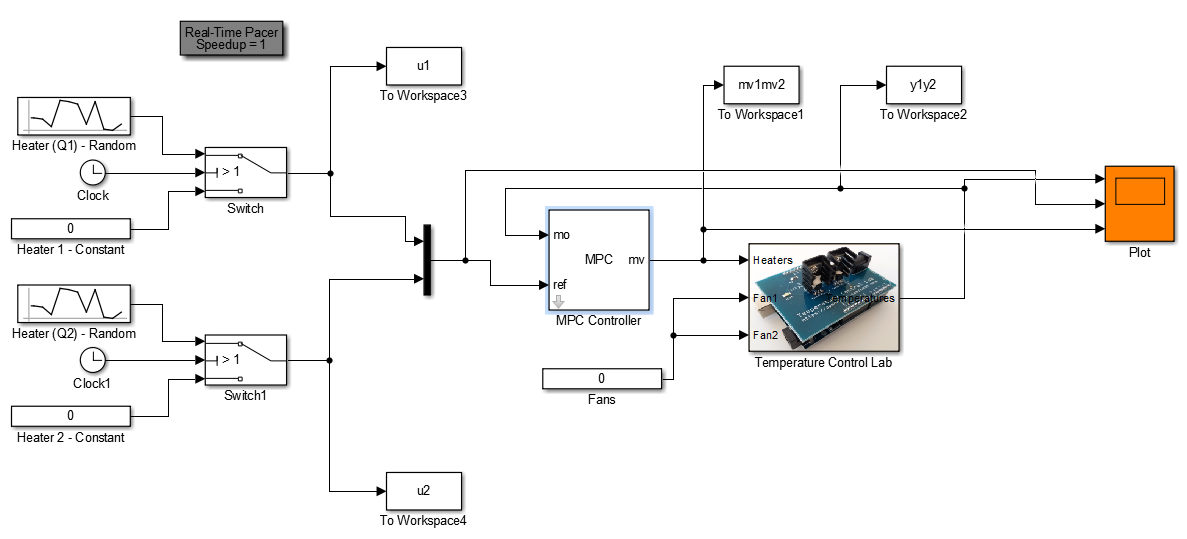
\includegraphics[width=1.00\textwidth]{./5_images/SimulinkUsingMPC.png} 
		\label{fig:simulinkusingmpc}
	\end{center}
	\centering
	\makebox[\width]{Fonte: Autor} 
\end{figure}

As \crefrange{fig:resultadosmpc-teoss}{fig:resultadosmpc-exparx} apresentam os gráficos de resposta em malha fechada
para cada um dos experimentos aplicando os modelos obtidos.

Para fins comparativos, a \cref{fig:resultadospid} apresenta o gráfico de resposta do controlador
\acrshort{pid} apresentado na \cref{sec:controlador_pid} e a \cref{tab:resultados_mpc_e_pid}
apresenta os valores de \textit{fit} (\cref{eq:nrmse}) dos controladores \acrshort{mpc} e \acrshort{pid} 
comparando-os com os sinais de referência (\textit{set-points}).

\begin{figure}[!h]
	\caption{Resposta do controlador MPC criado a partir do modelo teórico}
	\begin{center}
		\includegraphics[width=1.00\textwidth]{./5_images/ResultadosMPC-TeoSS.eps} 
		\label{fig:resultadosmpc-teoss}
	\end{center}
	\centering
	\makebox[\width]{Fonte: Autor} 
\end{figure}

\begin{figure}[!h]
	\caption{Resposta do controlador MPC criado a partir do modelo experimental (função de transferência)}
	\begin{center}
		\includegraphics[width=1.00\textwidth]{./5_images/ResultadosMPC-ExpTF.eps} 
		\label{fig:resultadosmpc-exptf}
	\end{center}
	\centering
	\makebox[\width]{Fonte: Autor} 
\end{figure}

\begin{figure}[!h]
	\caption{Resposta do controlador MPC criado a partir do modelo experimental (ARMAX)}
	\begin{center}
		\includegraphics[width=1.00\textwidth]{./5_images/ResultadosMPC-ExpARMAX.eps} 
		\label{fig:resultadosmpc-exparmax}
	\end{center}
	\centering
	\makebox[\width]{Fonte: Autor} 
\end{figure}

\begin{figure}[!h]
	\caption{Resposta do controlador MPC criado a partir do modelo experimental (Output-Error)}
	\begin{center}
		\includegraphics[width=1.00\textwidth]{./5_images/ResultadosMPC-ExpOE.eps} 
		\label{fig:resultadosmpc-expoe}
	\end{center}
	\centering
	\makebox[\width]{Fonte: Autor} 
\end{figure}

\begin{figure}[!h]
	\caption{Resposta do controlador MPC criado a partir do modelo experimental (espeço de estados)}
	\begin{center}
		\includegraphics[width=1.00\textwidth]{./5_images/ResultadosMPC-ExpSS.eps} 
		\label{fig:resultadosmpc-expss}
	\end{center}
	\centering
	\makebox[\width]{Fonte: Autor} 
\end{figure}

\begin{figure}[!h]
	\caption{Resposta do controlador MPC criado a partir do modelo experimental (ARX)}
	\begin{center}
		\includegraphics[width=1.00\textwidth]{./5_images/ResultadosMPC-ExpARX.eps} 
		\label{fig:resultadosmpc-exparx}
	\end{center}
	\centering
	\makebox[\width]{Fonte: Autor} 
\end{figure}

\begin{figure}[!h]
	\caption{Resposta do controlador PID auto-sintonizado}
	\begin{center}
		\includegraphics[width=1.00\textwidth]{./5_images/ResultadosPID.eps} 
		\label{fig:resultadospid}
	\end{center}
	\centering
	\makebox[\width]{Fonte: Autor} 
\end{figure}

\begin{table}[!h]
	\centering
	\caption{Qualidade dos controladores \acrshort{mpc} e \acrshort{pid}}
	\label{tab:resultados_mpc_e_pid}
	\begin{tabular}{l|cc|c} \toprule
		{Modelo utilizado no controlador}              			            &	{\textit{Fit} Sensor 1}	    &	{\textit{Fit} Sensor 2}     & {\textit{Fit} médio}			    \\ \midrule
		MPC Teórico \acrshort{ss} (\cref{eq:tclab_modelo_teorico})	        &   $45.84\%$                   &   $44.07\%$                   &   $44.95\%$                       \\ 
		MPC Experimental \acrshort{oe} (\cref{tab:tclabsp-model-oe})	    &   $44.35\%$                   &   $40.57\%$                   &   $42.46\%$                       \\ 
		MPC Experimental \acrshort{armax} (\cref{tab:tclabsp-model-armax})	&   $39.92\%$                   &   $42.50\%$                   &   $41.21\%$                       \\ 
		MPC Experimental \acrshort{tf} (\cref{tab:tclabsp-model-tf})		&   $40.25\%$                   &   $34.55\%$                   &   $37.40\%$                       \\ 
		MPC Experimental \acrshort{ss} (\cref{eq:tclabsp-model-ss})			&   $38.55\%$                   &   $33.57\%$                   &   $36.06\%$                       \\ 
		MPC Experimental \acrshort{arx}	(\cref{tab:tclabsp-model-arx})		&   $43.71\%$                   &   $27.33\%$                   &   $35.52\%$                       \\ 
		PID (\cref{tab:pid_values})	                                        &   $40.13\%$                   &   $26.44\%$                   &   $33.28\%$                       \\ \bottomrule 
	\end{tabular}
	\caption*{Fonte: Autor}
\end{table}

\chapter{Resultados e conclusões}
\label{ch:resultados}

A partir da \cref{tab:resultados_mpc_e_pid} é possível observar que dentre todos os controladores analisados,
o controlador \acrshort{mpc} criado a partir do modelo em espaço de estados e obtido por abordagem teórica
foi o aquele que mostrou melhor controle da planta estudada. Mesmo quando comparado com o controlador 
\acrshort{pid} de referência, o controle \acrshort{mpc} em questão mostrou uma maior velocidade para a estabilização
dos seus múltiplos sinais de saída. Contudo, vale ressaltar que este controlador \acrshort{pid} 
foi apenas sintonizado utilizando a função de \textit{auto-tunning} disponível no \acrshort{matlab}.
Um controlador \acrshort{pid} melhor parametrizado poderia ter uma performance muito mais próxima das 
performances obtidas nos controladores \acrshort{mpc}, pois segundo \citeonline{Shaaban2013} e
\citeonline{Taysom2017} a diferença na performance destes dois controles é muito pequena quando
a planta possui pouco ou nenhum atraso (como a planta utilizada neste estudo), porém quando os atrasos
na planta aumentam, a resposta do controlador \acrshort{pid} se degrada rapidamente.

Ainda comparando os controladores \acrshort{mpc} e \acrshort{pid}, além das performances de ambos poderem ser
diferenciadas devido ao atraso do sistema, \citeonline{Taysom2017} também aponta em seu estudo que os
controladores \acrshort{mpc} geralmente apresentam uma melhor resposta para sistemas \acrshort{mimo},
além de serem mais efetivos em sistemas onde os distúrbios podem ser modelados, uma vez que o
\acrshort{mpc} consegue utilizar o modelo do processo e o modelo do distúrbio conjuntamente para um 
controle mais assertivo. Em contrapartida os controladores \acrshort{pid} são relativamente mais
fáceis de sintonizar e muito mais fáceis de se implementar, além de possuírem resposta similar ao \acrshort{mpc}
em uma grande variedade de aplicações \cite{Taysom2017}.

Outro ponto de destaque para os controladores \acrshort{mpc} é a possibilidade da configuração de
restrições de atuação, algo que é impossível de se fazer utilizando um controle \acrshort{pid}.
No caso do uso de restrições, o controlador \acrshort{mpc} impede que a(s) saída(s) da planta controlada
ultrapassem limites indesejados, fazendo com que o \acrshort{mpc} seja uma opção de controle muito
interessante quando se deseja maximizar ou minimizar valores de produção sem que algumas variáveis
do processo atinjam ou ultrapassem limites indesejados.

Observa-se através das \crefrange{fig:resultadosmpc-exptf}{fig:resultadosmpc-exparx} que mesmo utilizando
uma metodologia consolidada academicamente para a criação do controle \acrshort{mpc} através de modelos
experimentais, a resposta em malha fechada pode não ser satisfatória. Nestas figuras é possível 
observar uma oscilação indesejada nas saídas da planta, além de erro estacionário em alguns casos.
Todavia, ferramentas como o \textit{MPC design} do \acrshort{matlab} podem auxiliar no desenvolvimento
de um controle \acrshort{mpc} através de um modelo experimental que ao ser empiricamente sintonizado
pode apresentar uma resposta satisfatória em malha fechada. A \cref{fig:resultadosmpcmanual-exptf}
apresenta o gráfico em malha fechada de um controlador \acrshort{mpc} utilizando o mesmo modelo experimental em
função de transferência apresentado no capítulo anterior, porém desta vez sintonizado empiricamente utilizando
a ferramenta \textit{MPC Design}. A \cref{tab:resultados_mpc_e_pid_e_manual} inclui este novo modelo 
na tabela já apresentada anteriormente e revela que, apesar de uma sintonia empírica, este controlador
apresenta uma aproximação do \textit{set-point} bem superior em comparação aos controladores baseados em 
modelos experimentais que já havíam sido apresentados neste trabalho.

\begin{figure}[!h]
	\caption{Resposta do controlador MPC criado empiricamente a partir do modelo experimental (função de transferência)}
	\begin{center}
		\includegraphics[width=1.00\textwidth]{./5_images/ResultadosMPCManual-ExpTF.eps} 
		\label{fig:resultadosmpcmanual-exptf}
	\end{center}
	\centering
	\makebox[\width]{Fonte: Autor} 
\end{figure}

\begin{table}[!h]
	\centering
	\caption{Qualidade do controlador \acrshort{mpc} sintonizado empiricamente}
	\label{tab:resultados_mpc_e_pid_e_manual}
	\begin{tabular}{l|cc|c} \toprule
		{Modelo utilizado no controlador}              			            &	{\textit{Fit} Sensor 1}	    &	{\textit{Fit} Sensor 2}     & {\textit{Fit} médio}			    \\ \midrule
		MPC Teórico \acrshort{ss} (\cref{eq:tclab_modelo_teorico})	        &   $45.84\%$                   &   $44.07\%$                   &   $44.95\%$                       \\ 
		\textbf{MPC Experimental \acrshort{tf} (empírico)}                  &   $\mathbf{46.46\%}$          &   $\mathbf{40.68\%}$          &   $\mathbf{43.57\%}$              \\ 
		MPC Experimental \acrshort{oe} (\cref{tab:tclabsp-model-oe})	    &   $44.35\%$                   &   $40.57\%$                   &   $42.46\%$                       \\ 
		MPC Experimental \acrshort{armax} (\cref{tab:tclabsp-model-armax})	&   $39.92\%$                   &   $42.50\%$                   &   $41.21\%$                       \\ 
		MPC Experimental \acrshort{tf} (\cref{tab:tclabsp-model-tf})		&   $40.25\%$                   &   $34.55\%$                   &   $37.40\%$                       \\ 
		MPC Experimental \acrshort{ss} (\cref{eq:tclabsp-model-ss})			&   $38.55\%$                   &   $33.57\%$                   &   $36.06\%$                       \\ 
		MPC Experimental \acrshort{arx}	(\cref{tab:tclabsp-model-arx})		&   $43.71\%$                   &   $27.33\%$                   &   $35.52\%$                       \\ 
		PID (\cref{tab:pid_values})	                                        &   $40.13\%$                   &   $26.44\%$                   &   $33.28\%$                       \\ \bottomrule 
	\end{tabular}
	\caption*{Fonte: Autor}
\end{table}

Nota-se também neste controlador\footnote{
    Parâmetros encontrados empiricamente e ajustados para este controlador: Tempo de amostragem ($t_s$) = 2s; Horizonte de predição = 120;
    Horizonte de Controle = 16; $\Delta$ = 0; R = 0,4393; Q = 0,2276.
} apresentado na \cref{fig:resultadosmpcmanual-exptf} uma maior estabilidade
das variáveis manipuladas, apesar de um \textit{overshoot} maior que os demais controles.

De forma geral é possível afirmar que os objetivos deste trabalho foram alcançados com êxito, uma vez que foi
possível desenvolver e implementar um controle \acrshort{mpc} na planta desejada, comparar este controle 
com um controle \acrshort{pid} convencional e ainda documentar todas as etapas de forma que essas possam ser reproduzidas
por outros estudantes que estejam pesquisando sobre o \acrlong{mpc}.

% Comentários do Brincalepe
% TODO Falar de possíveis melhorias futuras. (Sintonizar melhor o PID, Alterar a planta para ter atraso, modelar ruido, etc)
% TODO Detalhar MPC Design. Como foi feita a simulação empírica
% TODO Avaliar se vale a pena alterar a função FIT por IAE (integral absolute error) 
% TODO Fazer versão digital de lado único para a defesa.


% \chapter{Cronograma}
\label{ch:cronograma}

\begin{table}[h]
	\centering
	\caption{Cronograma de trabalho}
	\label{tab:cronograma}
	\begin{tabular}{lccccc} \toprule
		{Atividade} 	                & {Jul-19}	& {Ago-19}	& {Set-19}  & {Out-19}  & {Nov-19}  \\ \midrule
        Modelagem experimental          & X         &           &           &           &           \\
        Desenvolvimento do controlador  & X         & X         & X         &           &           \\
        Análise de resultados	        &           &           & X         & X         &           \\
        Ajuste de dissertação           &           &           &           &           & X        	\\ \bottomrule
	\end{tabular}
	\caption*{Fonte: Autor}
\end{table}


% ELEMENTOS PÓS-TEXTUAIS
\postextual

% Referências bibliográficas
\bibliography{./3_posText/library}

% Glossário
% Consulte o manual da classe abntex2 para orientações sobre o glossário.
% % ----------------------------------------------------------
% Glossário
% ----------------------------------------------------------

% ---
% Define nome e preâmbulo do glossário
% ---
\phantompart
%\renewcommand{\glossaryname}{Glossário}  A opção babel do glossaries faz a tradução.
\renewcommand{\glossarypreamble}{Esta é a descrição do glossário. Experimente
visualizar outros estilos de glossários, como o \texttt{altlisthypergroup},
por exemplo.\\
\\}

% ---
% Traduções para o ambiente glossaries
% ---  
% A opção babel do glossaries faz a tradução.

%\providetranslation{Glossary}{Glossário}
%\providetranslation{Acronyms}{Siglas}
%\providetranslation{Notation (glossaries)}{Notação}
%\providetranslation{Description (glossaries)}{Descrição}
%\providetranslation{Symbol (glossaries)}{Símbolo}
%\providetranslation{Page List (glossaries)}{Lista de Páginas}
%\providetranslation{Symbols (glossaries)}{Símbolos}
%\providetranslation{Numbers (glossaries)}{Números} 
% ---

% ---
% Estilo de glossário
% ---
% \setglossarystyle{index}
% \setglossarystyle{altlisthypergroup}
 \setglossarystyle{tree}  % Já selecionado no arquivo .sty 


% ---
% Imprime o glossário
% ---
\cleardoublepage
\phantomsection
\addcontentsline{toc}{chapter}{\glossaryname}
\printglossaries % imprime todas as entradas

\imprimirglossario  % não imprime acronimos (siglas) e nem simbolos
% ---

% Apêndices
\begin{apendicesenv}

% Imprime uma página indicando o início dos apêndices
\partapendices

% =====================================================================================================
% ============================================= Chapter ===============================================
% =====================================================================================================
\chapter{Códigos-fonte}
\label{ch:codigos_extras}

\section{Método de pesquisa em grade}

\lstinputlisting[	
	caption={Pesquisa em grade com número escalar},
	captionpos=t,
	label={lst:grid_search_scalar},
	language=Python,
	style=Python_lang]
	{./4_Codes/grid_search_scalar.py}
	\begin{center}
		\makebox[\width]{Fonte: Autor, adaptado de \citeonline{Haugen2018}}
	\end{center}

\section{Método de pesquisa em grade com duas variáveis}

\lstinputlisting[	
	caption={Pesquisa em grade com duas variáveis},
	captionpos=t,
	label={lst:grid_search_vectorial},
	language=Python,
	style=Python_lang]
	{./4_Codes/grid_search_vectorial.py}
	\begin{center}
		\makebox[\width]{Fonte: Autor, adaptado de \citeonline{Haugen2018}}
	\end{center}

\section{Exemplo do método \acrlong{mhe}}

% (Brincalepe): O código da página 44 deve ser deslocado para o apêndice.
% (cont.) Se quiser, destaque apenas alguma parte mais relevante e mantenha no corpo do texto.
\lstinputlisting[	
	caption={Exemplo do método \acrlong{mhe}},
	captionpos=t,
	label={lst:mhe_example},
	language=Python,
	style=Python_lang]
	{./4_Codes/mhe_example.py}
	\begin{center}
		\makebox[\width]{Fonte: Autor, adaptado de \citeonline{Haugen2018}}
	\end{center}

\section{Exemplo de aplicação do \acrlong{mpc}}

\lstinputlisting[	
	caption={Exemplo de aplicação do \acrlong{mpc}},
	captionpos=t,
	label={lst:mpc_example},
	language=Python,
	style=Python_lang]
	{./4_Codes/mpc_example.py}
	\begin{center}
		\makebox[\width]{Fonte: Autor, adaptado de \citeonline{Haugen2018}}
	\end{center}
% (Brincalepe): O código da página 58 também pode ser deslocado para o Apêndice.
% (cont.) Seria interessante descrevê-lo no corpo de texto através de um diagrama.

% =====================================================================================================
% ============================================= Chapter ===============================================
% =====================================================================================================
\chapter{Escolha da frequência de amostragem utilizando autocovariância}
\label{ch:sampling_time_using_autocorrelation}

A regra prática para a escolha da frequência de amostragem de sinal descrita por \citeonline{Aguirre2015}
e citada na \cref{subsubsec:periodo_de_amostragem} pode nem sempre ajudar muito, uma vez que é possível
que não se tenha nenhum conhecimento prévio do sinal para poder aplicar a regra de escolher uma frequência
de 5 a 10 vezes maior que a frequência de interesse \cite{Aguirre2015}. Para casos assim, \citeonline{Aguirre2015}
descreve uma outra técnica, que será apresentada nos parágrafos a seguir. 

Assume-se que o sinal já amostrado, $y^*(k)$, tenha sido obtido utilizando-se um tempo
de amostragem muito pequeno, ou seja, o sinal está superamostrado. Sendo assim, deseja-se encontrar o
valor $\Delta$ que descreva a fração pela qual o $y^*(k)$ pode ser decimado a fim de obter um sinal de trabalho
$y(k) = y^*(\Delta k)$, ou seja, o sinal decimado que ainda mantem as características originais do sinal $y^*(k)$.

Para fazer isso é necessário verificar o nível de correlação entre observações adjacentes do sinal
$y^*(k)$. Quanto mais superamostrado estiver o sinal $y^*(k)$, maior será a redundância entre duas
observações consecutivas. Este nível de correlação pode ser obtido calculando as funções de
autocovariância linear e não-linear (mostradas na \cref{eq:autocorrelation}) do sinal original.

\begin{subequations}
    \label{eq:autocorrelation}
    \begin{align}
		r_{y^*}(\tau) &= \mathrm{E} \left[(y^*(k) - \overline{y^*(k)}) (y^*(k - \tau) - \overline{y^*(k)})\right]		\\
		r_{y^{*2'}}(\tau) &= \mathrm{E} \left[(y^{*2}(k) - \overline{y^{*2}(k)}) (y^{*2}(k - \tau) - \overline{y^{*2}(k)})\right]
    \end{align}
\end{subequations}

$\mathrm{E}[\cdot]$ indica a esperança matemática, porém, sendo $y^*(k)$ ergótico, $\mathrm{E}[\cdot]$
pode ser substituída pela média temporal.

Após calculados $r_{y^*}(\tau)$ e $r_{y^{*2'}}(\tau)$, determinam-se seus primeiros mínimos,
$\tau_{y^*}$ e $\tau_{y^{*2'}}$, respectivamente. O menor desses mínimos passa a ser o valor de trabalho
$\tau_{m}^{*}$, ou seja, $\tau_{m}^{*} = \mathrm{min} \left[ \tau_{y^*} , \tau_{y^{*2'}} \right]$.

Por fim, deseja-se escolha $\Delta$ de forma que as funções de autocovariância do sinal decimado $y(k) = y^*(k)$
satisfaçam

\begin{equation}
    \label{eq:tau_m}
    10 \leq \tau_m \leq 20
\end{equation}

\noindent
sendo que $\tau_m$ é definido pelo sinal decimado $y(k)$ de maneira análoga a $\tau_m^*$ para o
sinal $y^*(k)$. Os limites inferior e superior da \cref{eq:tau_m} podem ser relaxados para
$5$ e $10$, respectivamente.

% =====================================================================================================
% ============================================= Section ===============================================
% =====================================================================================================
\section{Aplicação prática}
\label{ch:using_sampling_time_with_autocorrelation}

As \cref{fig:rise_time_sensor1,fig:rise_time_sensor2} da \cref{subsubsec:periodo_de_amostragem}
apresentam a resposta dos sensores de temperatura do \acrshort{tclabsp} quando o Aquecedor 1 é
excitado com um degrau de 0 à 50\%.

Após alguns testes preliminares, foi observado que o sistema apresentava uma resposta lenta
e que, portanto, uma coleta de dados com tempo de amostragem de $0.25s$ seria suficiente para
superamostrar os dados e garantir que todas as características de resposta do sistema tenham
sido amostradas.

Calcula-se então as funções de autocovariância apresentadas na \cref{eq:autocorrelation} para os
sensores de temperatura 1 e 2, como apresentado na \cref{fig:autocorrelationS1S2}.

\begin{figure}[h]
	\caption{Funções de autocovariância dos Sensores de Temperatura 1 e 2}
	\begin{center}
		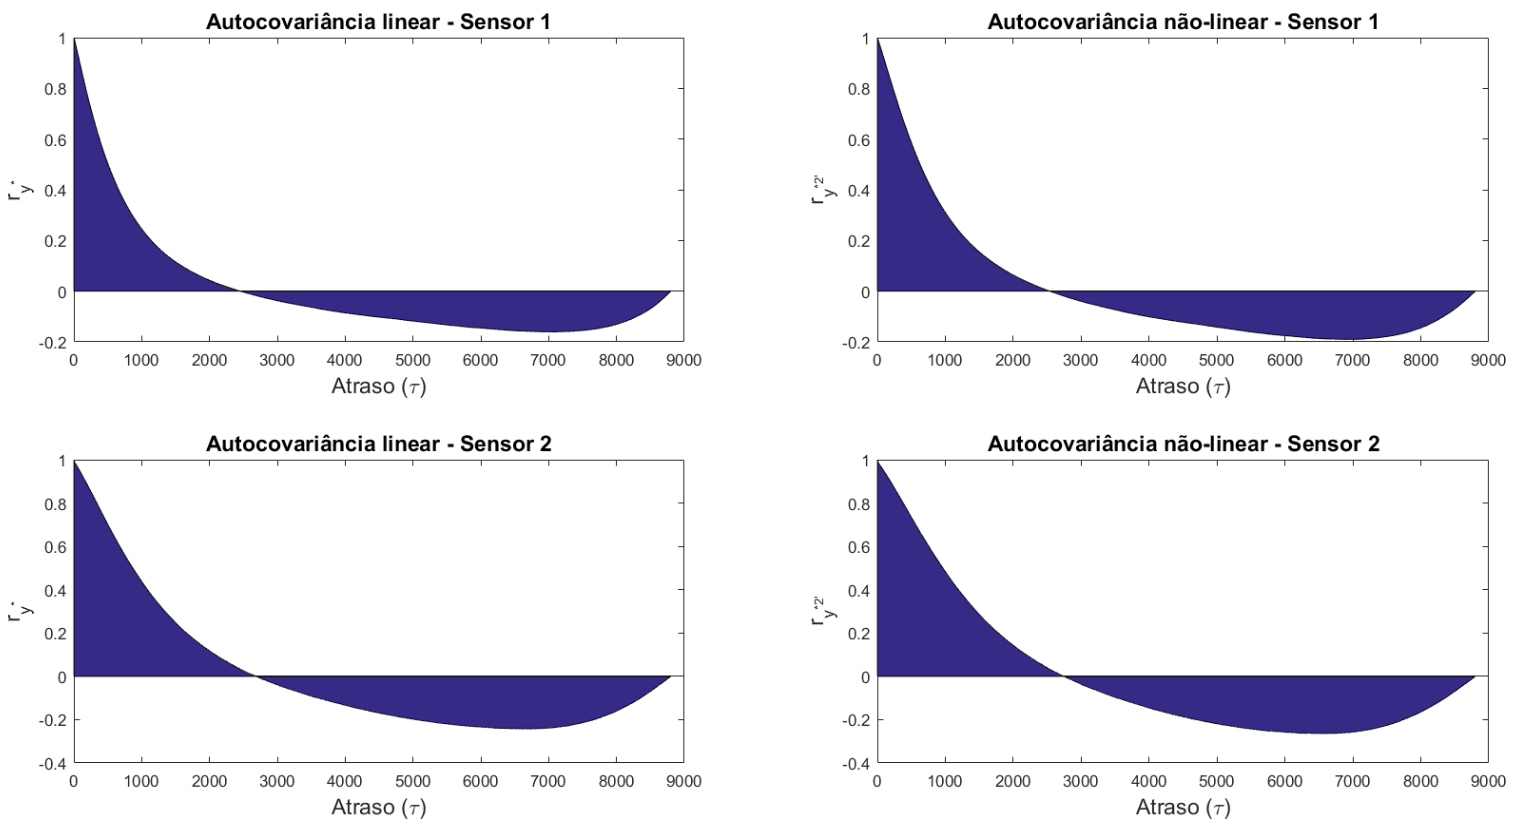
\includegraphics[width=0.95\textwidth]{./5_images/AutocorrelationS1S2.png} 
		\label{fig:autocorrelationS1S2}
	\end{center}
	\centering
	\makebox[\width]{Fonte: \citeonline{Prata2019}} 
\end{figure}

Para cada um dos sensores, encontramos então o valor mínimo das funções de autocovariância
($\tau_{y^{*}}$ e $\tau_{y^{*2'}}$), e a partir delas determinamos $\tau_m^*$
($\tau_{m}^{*} = \mathrm{min} \left[ \tau_{y^*} , \tau_{y^{*2'}} \right]$).
O resultado é apresentado na \cref{tab:tau_s1s2}.

\begin{table}[h]
	\centering
	\caption{Mínimos das funções de autocovariância}
	\label{tab:tau_s1s2}
	\begin{tabular}{llll} \toprule
		{Sensor}		& {$\tau_{y^{*}}$}		& {$\tau_{y^{*2'}}$}		& {$\pmb{\tau}_{\pmb{m}}^{\pmb{*}}$}		\\ \midrule
		Sensor 1		& $7015$				& $6925$					& $\pmb{6}\pmb{9}\pmb{2}\pmb{5}$			\\
		Sensor 2		& $6735$				& $6621$					& $\pmb{6}\pmb{6}\pmb{2}\pmb{1}$			\\ \bottomrule
	\end{tabular}
	\caption*{Fonte: Autor}
\end{table}

Conhecendo $\tau_{m}^{*}$ é possível encontrar um valor de $\Delta$ para obter o sinal decimado
$y(k) = y^*(\Delta k)$, tal que o valor mínimo da suas funções de autocovariância satisfaçam
\cref{eq:tau_m}.

Uma demonstração do efeito da variação do $\Delta$ no tempo de amostragem do sinal
pode ver vista na \cref{tab:delta_action}

\begin{table}[h]
	\centering
	\caption{Efeito do $\Delta$ no tempo de amostragem}
	\label{tab:delta_action}
	\begin{tabular}{cccccc} \toprule
		{k}		& {$\Delta=1$}		& {$\Delta=2$}		& {$\cdots$}	& {$\Delta=4$}	& {$\cdots$} 	\\ \midrule
		1		& $0.00$			& $0.00$			& \hfill		& $0.00$		& \hfill		\\
		2		& $0.25$			& $0.50$			& \hfill		& $1.00$		& \hfill		\\
		3		& $0.50$			& $1.00$			& \hfill		& $2.00$		& \hfill		\\
		4		& $0.75$			& $0.50$			& \hfill		& $3.00$		& \hfill		\\
		5		& $1.00$			& $2.00$			& \hfill		& $4.00$		& \hfill		\\ \bottomrule 
	\end{tabular}
	\caption*{Fonte: Autor}
\end{table}

Através de um algoritmo\footnote{
	Indicar algoritmo utilizado			% TODO Indicar algoritmo utilizado
} foi possível testar diferentes valores de $\Delta$ a fim de encontrar
aquele que primeiro satisfizesse a \cref{eq:tau_m}, e por meio deste algoritmo encontrou-se
os valores de $\Delta$ e de $T_s$ (tempo de amostragem) indicados da \cref{eq:delta_and_ts}.

\begin{subequations}
    \label{eq:delta_and_ts}
    \begin{align}
		\Delta &= 253	\\
		T_s &= 63.25s
    \end{align}
\end{subequations}


\end{apendicesenv}


% Anexos
% \begin{anexosenv}

% Imprime uma página indicando o início dos anexos
\partanexos

\chapter{fmincon}
\label{ch:fmincon}

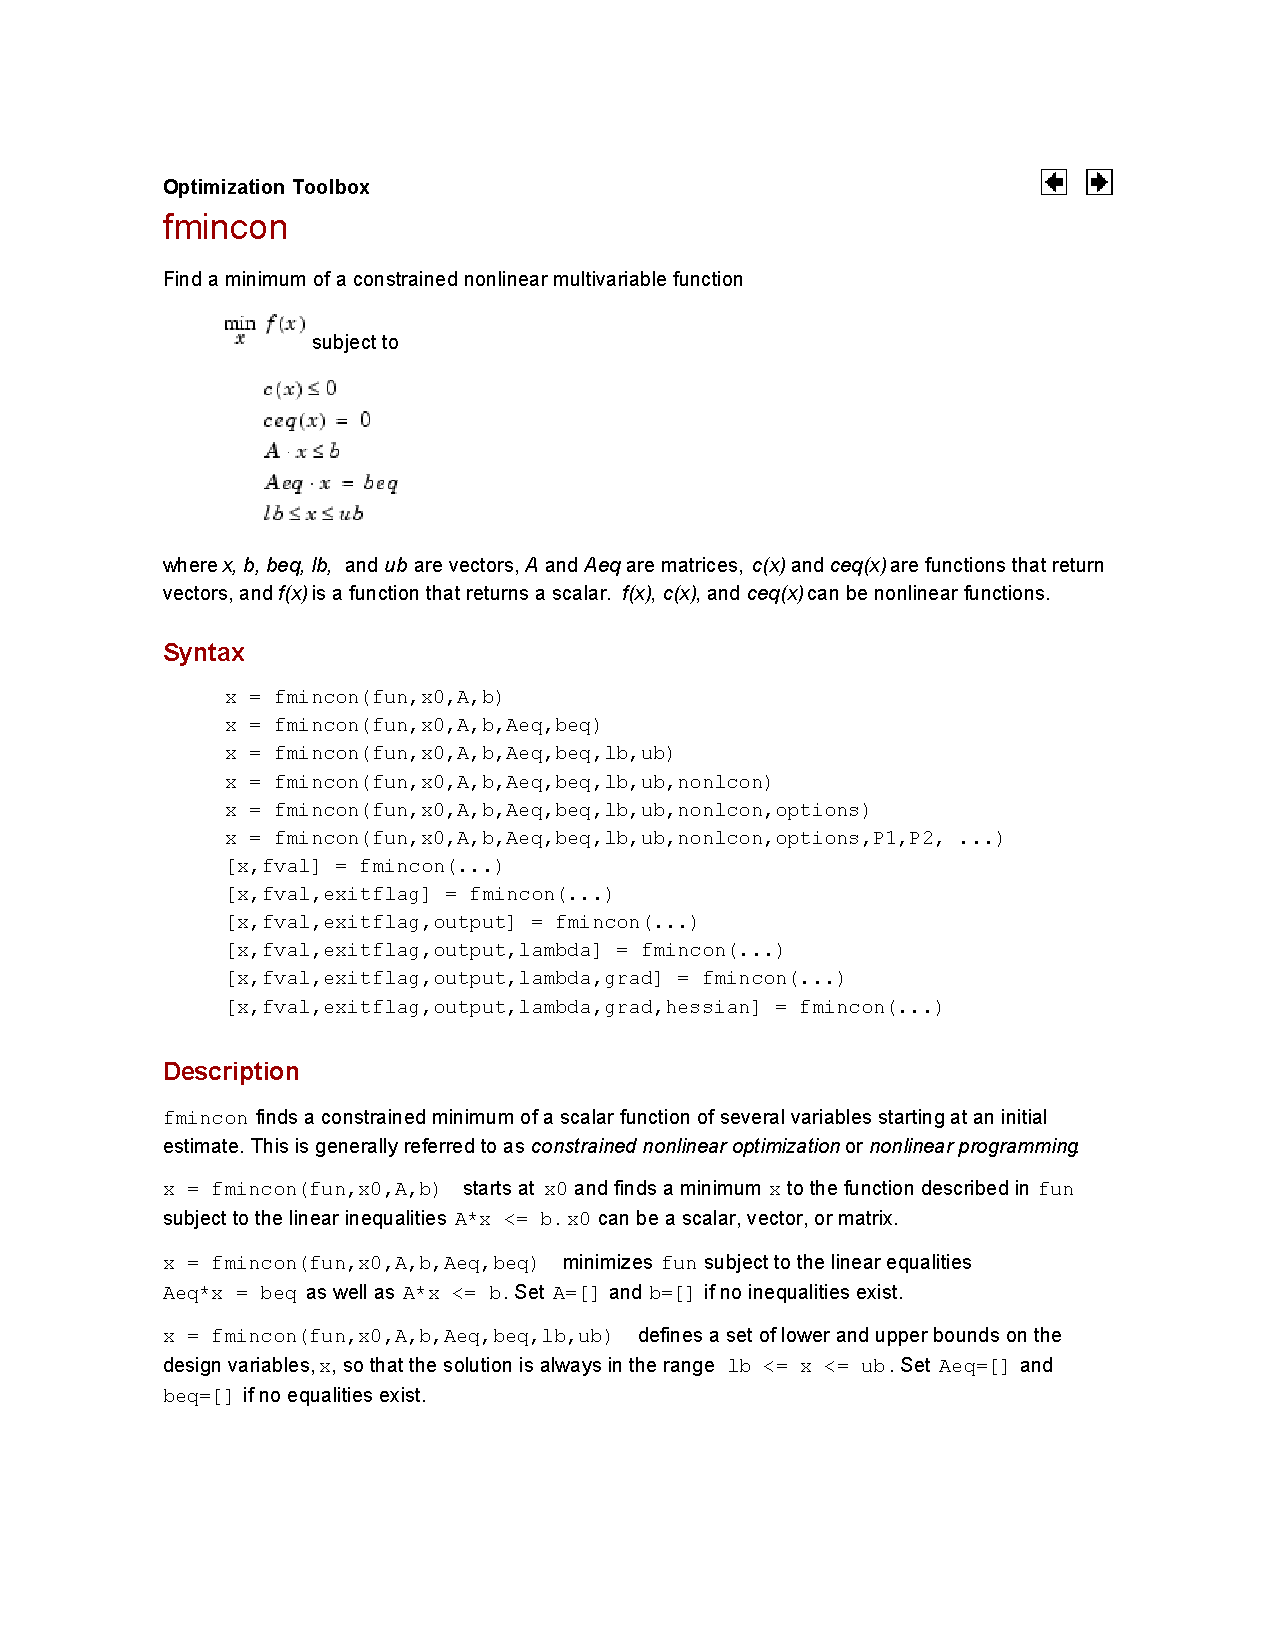
\includepdf[pages=-]{6_annex/fmincon.pdf}

\chapter{scipy.optimize.minimize}
\label{ch:scipy_optimize_minimize}

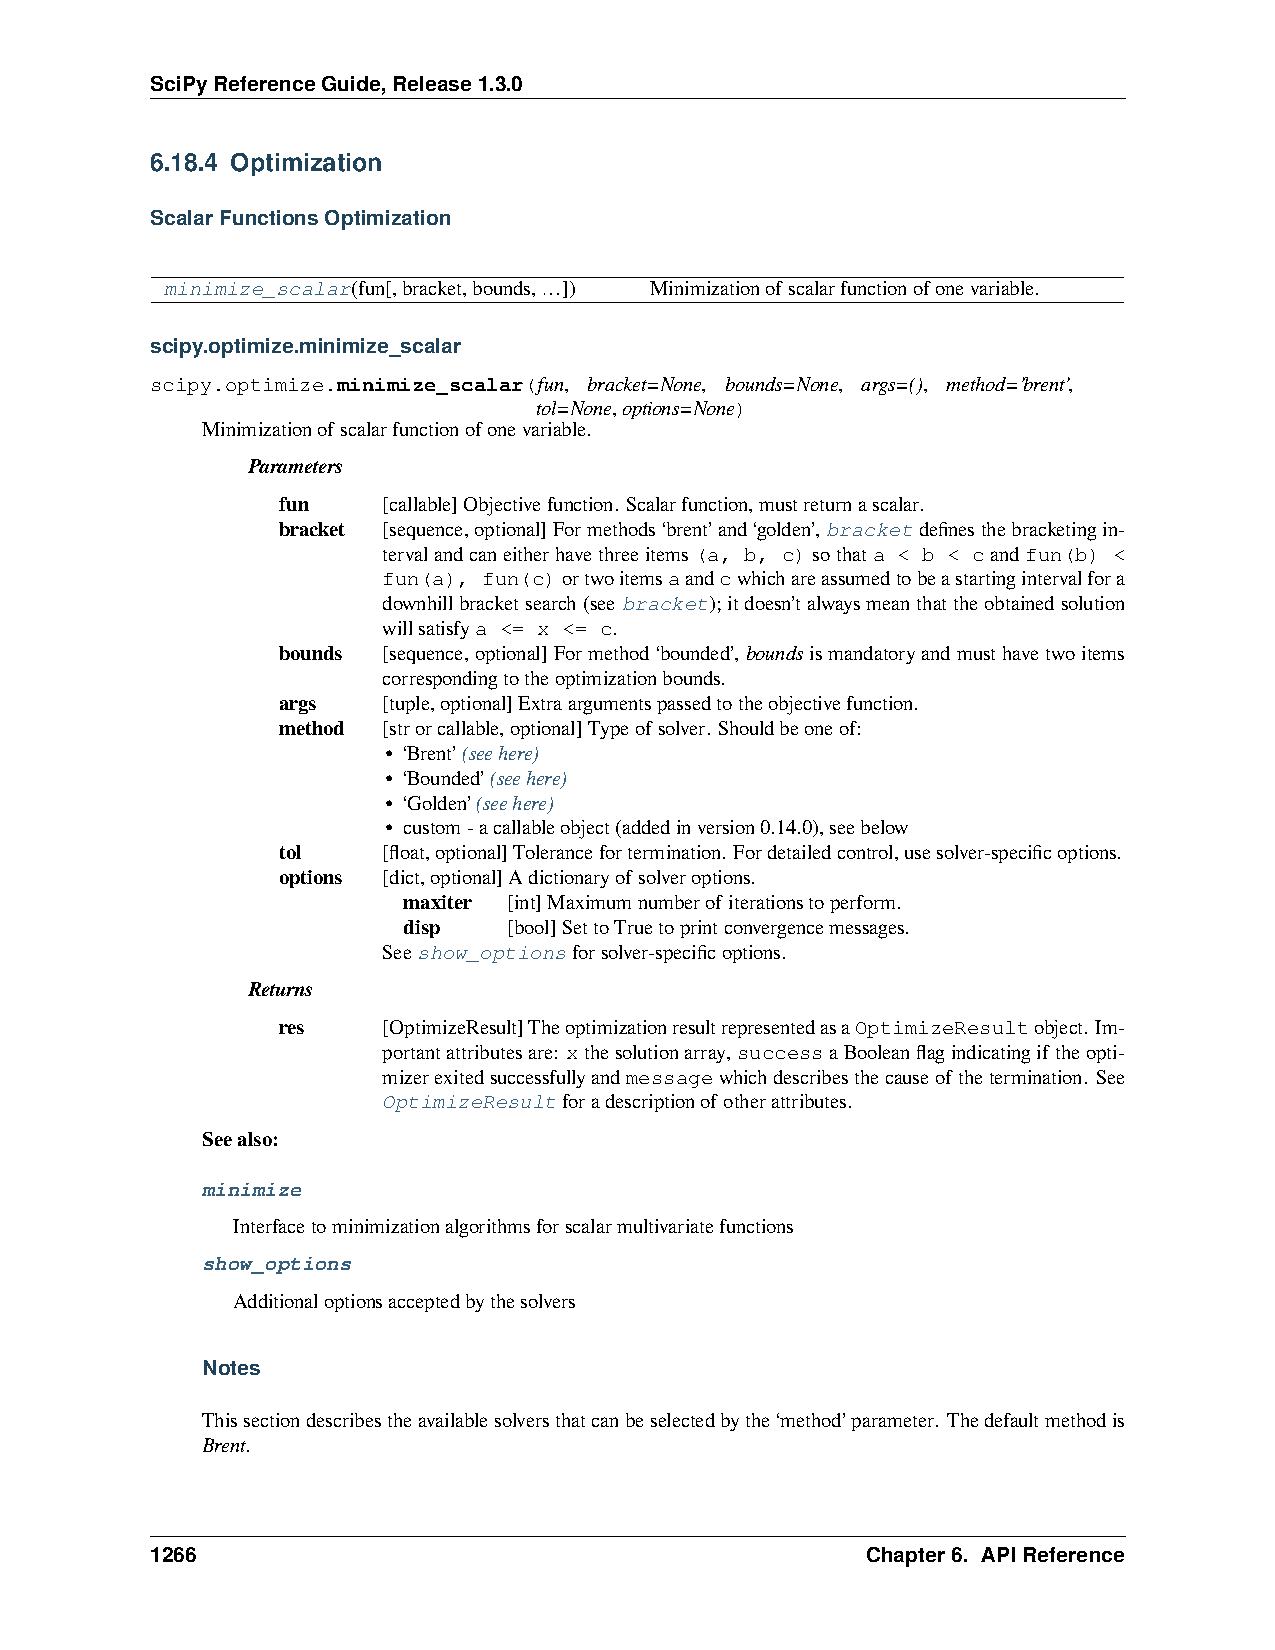
\includepdf[pages=-]{6_annex/scipy_optimize_minimize.pdf}


\end{anexosenv}


% ÍNDICE REMISSIVO
\phantompart
\printindex

\end{document}
